\chapter{Introduction}\label{chap:intro}
% This thesis is about Bayesian optimization. The main topic is the derivation of an upper bound on the chance of further improvement in such a scheme.
% \textcolor{red}{Satz rauslassen?}
% % In order to discuss Bayesian optimization, the first half of this thesis will be dedicated to the neccessary probability theory foundations, some stochastical tools and Gaussian process regression.
%
%
\section{Topic of this Thesis}
% \section*{Optimization}
Let us start by looking at a generic optimization problem. That is, we have some function \( f \colon \mathcal{X} \to \mathbb{R} \) on a suitable space $\mathcal{X}$, and we want to find a minimizer
\[
    x^{*} \in \argmin_{x \in \mathcal{X}} f(x).
\]
An example of such a function is shown in \cref{fig:optimization_intro}.
One simple way to approach this problem would be to start checking points randomly and remembering the lowest point we encountered. 
For finite spaces $\mathcal{X}$ this is sometimes feasible, but quickly runs into limitations if the number of elements gets too large.
% 
An example of a more refined strategy would be to use information of a lower bound on the function, if we have one. 
This lets us rule out areas of search, where the lower bound is already higher than a value we have previously encountered, and subsequently only look in areas, in which improvement is possible. 
This method is called branch and bound~\cite{lawler1966branch}.
Although this is an improvement on the previous method, it still does not guarantee, that we will find the global minimum.
% 
But it does show a common theme in optimization of using all the availaible information about the space and the objective function to our benefit. Is the function differentiable? Linear? Is the space discrete? Is it continous, but still finite dimensional? These, among many others, are restrictions with specific approaches taylored to them. The approach discussed in this thesis is no different. 
\begin{figure}[H]
    \centering
    %% Creator: Matplotlib, PGF backend
%%
%% To include the figure in your LaTeX document, write
%%   \input{<filename>.pgf}
%%
%% Make sure the required packages are loaded in your preamble
%%   \usepackage{pgf}
%%
%% Also ensure that all the required font packages are loaded; for instance,
%% the lmodern package is sometimes necessary when using math font.
%%   \usepackage{lmodern}
%%
%% Figures using additional raster images can only be included by \input if
%% they are in the same directory as the main LaTeX file. For loading figures
%% from other directories you can use the `import` package
%%   \usepackage{import}
%%
%% and then include the figures with
%%   \import{<path to file>}{<filename>.pgf}
%%
%% Matplotlib used the following preamble
%%   \def\mathdefault#1{#1}
%%   \everymath=\expandafter{\the\everymath\displaystyle}
%%   \usepackage[T1]{fontenc}
%%   \usepackage{siunitx}
%%   \usepackage{amssymb}
%%   \usepackage{amsmath}
%%   \makeatletter\@ifpackageloaded{underscore}{}{\usepackage[strings]{underscore}}\makeatother
%%
\begingroup%
\makeatletter%
\begin{pgfpicture}%
\pgfpathrectangle{\pgfpointorigin}{\pgfqpoint{3.473106in}{1.287899in}}%
\pgfusepath{use as bounding box, clip}%
\begin{pgfscope}%
\pgfsetbuttcap%
\pgfsetmiterjoin%
\definecolor{currentfill}{rgb}{1.000000,1.000000,1.000000}%
\pgfsetfillcolor{currentfill}%
\pgfsetlinewidth{0.000000pt}%
\definecolor{currentstroke}{rgb}{1.000000,1.000000,1.000000}%
\pgfsetstrokecolor{currentstroke}%
\pgfsetdash{}{0pt}%
\pgfpathmoveto{\pgfqpoint{0.000000in}{0.000000in}}%
\pgfpathlineto{\pgfqpoint{3.473106in}{0.000000in}}%
\pgfpathlineto{\pgfqpoint{3.473106in}{1.287899in}}%
\pgfpathlineto{\pgfqpoint{0.000000in}{1.287899in}}%
\pgfpathlineto{\pgfqpoint{0.000000in}{0.000000in}}%
\pgfpathclose%
\pgfusepath{fill}%
\end{pgfscope}%
\begin{pgfscope}%
\pgfsetbuttcap%
\pgfsetmiterjoin%
\definecolor{currentfill}{rgb}{1.000000,1.000000,1.000000}%
\pgfsetfillcolor{currentfill}%
\pgfsetlinewidth{0.000000pt}%
\definecolor{currentstroke}{rgb}{0.000000,0.000000,0.000000}%
\pgfsetstrokecolor{currentstroke}%
\pgfsetstrokeopacity{0.000000}%
\pgfsetdash{}{0pt}%
\pgfpathmoveto{\pgfqpoint{0.000000in}{0.000000in}}%
\pgfpathlineto{\pgfqpoint{3.473106in}{0.000000in}}%
\pgfpathlineto{\pgfqpoint{3.473106in}{1.287899in}}%
\pgfpathlineto{\pgfqpoint{0.000000in}{1.287899in}}%
\pgfpathlineto{\pgfqpoint{0.000000in}{0.000000in}}%
\pgfpathclose%
\pgfusepath{fill}%
\end{pgfscope}%
\begin{pgfscope}%
\pgfpathrectangle{\pgfqpoint{0.000000in}{0.000000in}}{\pgfqpoint{3.473106in}{1.287899in}}%
\pgfusepath{clip}%
\pgfsetrectcap%
\pgfsetroundjoin%
\pgfsetlinewidth{1.505625pt}%
\definecolor{currentstroke}{rgb}{0.149020,0.274510,0.325490}%
\pgfsetstrokecolor{currentstroke}%
\pgfsetdash{}{0pt}%
\pgfpathmoveto{\pgfqpoint{0.157868in}{1.229358in}}%
\pgfpathlineto{\pgfqpoint{0.192634in}{1.146241in}}%
\pgfpathlineto{\pgfqpoint{0.284290in}{0.923314in}}%
\pgfpathlineto{\pgfqpoint{0.309574in}{0.869211in}}%
\pgfpathlineto{\pgfqpoint{0.331698in}{0.827275in}}%
\pgfpathlineto{\pgfqpoint{0.350661in}{0.796130in}}%
\pgfpathlineto{\pgfqpoint{0.366463in}{0.773921in}}%
\pgfpathlineto{\pgfqpoint{0.382266in}{0.755307in}}%
\pgfpathlineto{\pgfqpoint{0.398069in}{0.740370in}}%
\pgfpathlineto{\pgfqpoint{0.410711in}{0.731066in}}%
\pgfpathlineto{\pgfqpoint{0.423353in}{0.724062in}}%
\pgfpathlineto{\pgfqpoint{0.435995in}{0.719272in}}%
\pgfpathlineto{\pgfqpoint{0.448637in}{0.716573in}}%
\pgfpathlineto{\pgfqpoint{0.461279in}{0.715806in}}%
\pgfpathlineto{\pgfqpoint{0.477082in}{0.717276in}}%
\pgfpathlineto{\pgfqpoint{0.492885in}{0.721038in}}%
\pgfpathlineto{\pgfqpoint{0.511848in}{0.727896in}}%
\pgfpathlineto{\pgfqpoint{0.540293in}{0.741053in}}%
\pgfpathlineto{\pgfqpoint{0.581379in}{0.760196in}}%
\pgfpathlineto{\pgfqpoint{0.600343in}{0.766790in}}%
\pgfpathlineto{\pgfqpoint{0.616145in}{0.770350in}}%
\pgfpathlineto{\pgfqpoint{0.631948in}{0.771715in}}%
\pgfpathlineto{\pgfqpoint{0.647751in}{0.770543in}}%
\pgfpathlineto{\pgfqpoint{0.660393in}{0.767599in}}%
\pgfpathlineto{\pgfqpoint{0.673035in}{0.762761in}}%
\pgfpathlineto{\pgfqpoint{0.685677in}{0.755963in}}%
\pgfpathlineto{\pgfqpoint{0.701480in}{0.744666in}}%
\pgfpathlineto{\pgfqpoint{0.717282in}{0.730274in}}%
\pgfpathlineto{\pgfqpoint{0.733085in}{0.712880in}}%
\pgfpathlineto{\pgfqpoint{0.752048in}{0.688289in}}%
\pgfpathlineto{\pgfqpoint{0.771011in}{0.660049in}}%
\pgfpathlineto{\pgfqpoint{0.793135in}{0.623229in}}%
\pgfpathlineto{\pgfqpoint{0.821580in}{0.571392in}}%
\pgfpathlineto{\pgfqpoint{0.919556in}{0.388475in}}%
\pgfpathlineto{\pgfqpoint{0.941680in}{0.353405in}}%
\pgfpathlineto{\pgfqpoint{0.960643in}{0.326811in}}%
\pgfpathlineto{\pgfqpoint{0.979606in}{0.303867in}}%
\pgfpathlineto{\pgfqpoint{0.995409in}{0.287760in}}%
\pgfpathlineto{\pgfqpoint{1.011211in}{0.274520in}}%
\pgfpathlineto{\pgfqpoint{1.027014in}{0.264204in}}%
\pgfpathlineto{\pgfqpoint{1.042817in}{0.256815in}}%
\pgfpathlineto{\pgfqpoint{1.058619in}{0.252299in}}%
\pgfpathlineto{\pgfqpoint{1.074422in}{0.250554in}}%
\pgfpathlineto{\pgfqpoint{1.090225in}{0.251429in}}%
\pgfpathlineto{\pgfqpoint{1.106027in}{0.254731in}}%
\pgfpathlineto{\pgfqpoint{1.121830in}{0.260230in}}%
\pgfpathlineto{\pgfqpoint{1.140793in}{0.269362in}}%
\pgfpathlineto{\pgfqpoint{1.162917in}{0.282879in}}%
\pgfpathlineto{\pgfqpoint{1.188201in}{0.301065in}}%
\pgfpathlineto{\pgfqpoint{1.235609in}{0.338645in}}%
\pgfpathlineto{\pgfqpoint{1.273535in}{0.367359in}}%
\pgfpathlineto{\pgfqpoint{1.298820in}{0.383805in}}%
\pgfpathlineto{\pgfqpoint{1.320943in}{0.395585in}}%
\pgfpathlineto{\pgfqpoint{1.339907in}{0.403361in}}%
\pgfpathlineto{\pgfqpoint{1.358870in}{0.408754in}}%
\pgfpathlineto{\pgfqpoint{1.377833in}{0.411603in}}%
\pgfpathlineto{\pgfqpoint{1.396796in}{0.411814in}}%
\pgfpathlineto{\pgfqpoint{1.415759in}{0.409359in}}%
\pgfpathlineto{\pgfqpoint{1.434722in}{0.404268in}}%
\pgfpathlineto{\pgfqpoint{1.453686in}{0.396630in}}%
\pgfpathlineto{\pgfqpoint{1.472649in}{0.386584in}}%
\pgfpathlineto{\pgfqpoint{1.494772in}{0.372066in}}%
\pgfpathlineto{\pgfqpoint{1.516896in}{0.354877in}}%
\pgfpathlineto{\pgfqpoint{1.542180in}{0.332492in}}%
\pgfpathlineto{\pgfqpoint{1.573786in}{0.301394in}}%
\pgfpathlineto{\pgfqpoint{1.621194in}{0.251141in}}%
\pgfpathlineto{\pgfqpoint{1.684404in}{0.184594in}}%
\pgfpathlineto{\pgfqpoint{1.719170in}{0.151406in}}%
\pgfpathlineto{\pgfqpoint{1.747615in}{0.127241in}}%
\pgfpathlineto{\pgfqpoint{1.772899in}{0.108492in}}%
\pgfpathlineto{\pgfqpoint{1.798183in}{0.092604in}}%
\pgfpathlineto{\pgfqpoint{1.820307in}{0.081199in}}%
\pgfpathlineto{\pgfqpoint{1.842431in}{0.072201in}}%
\pgfpathlineto{\pgfqpoint{1.864554in}{0.065634in}}%
\pgfpathlineto{\pgfqpoint{1.886678in}{0.061478in}}%
\pgfpathlineto{\pgfqpoint{1.908802in}{0.059673in}}%
\pgfpathlineto{\pgfqpoint{1.930926in}{0.060123in}}%
\pgfpathlineto{\pgfqpoint{1.953049in}{0.062704in}}%
\pgfpathlineto{\pgfqpoint{1.978334in}{0.068069in}}%
\pgfpathlineto{\pgfqpoint{2.003618in}{0.075765in}}%
\pgfpathlineto{\pgfqpoint{2.032063in}{0.086862in}}%
\pgfpathlineto{\pgfqpoint{2.063668in}{0.101726in}}%
\pgfpathlineto{\pgfqpoint{2.101594in}{0.122286in}}%
\pgfpathlineto{\pgfqpoint{2.149002in}{0.150729in}}%
\pgfpathlineto{\pgfqpoint{2.300708in}{0.243785in}}%
\pgfpathlineto{\pgfqpoint{2.344955in}{0.267469in}}%
\pgfpathlineto{\pgfqpoint{2.386042in}{0.287079in}}%
\pgfpathlineto{\pgfqpoint{2.427129in}{0.304173in}}%
\pgfpathlineto{\pgfqpoint{2.465055in}{0.317652in}}%
\pgfpathlineto{\pgfqpoint{2.502981in}{0.328947in}}%
\pgfpathlineto{\pgfqpoint{2.544068in}{0.338828in}}%
\pgfpathlineto{\pgfqpoint{2.585155in}{0.346438in}}%
\pgfpathlineto{\pgfqpoint{2.629403in}{0.352362in}}%
\pgfpathlineto{\pgfqpoint{2.676811in}{0.356459in}}%
\pgfpathlineto{\pgfqpoint{2.730540in}{0.358815in}}%
\pgfpathlineto{\pgfqpoint{2.793750in}{0.359274in}}%
\pgfpathlineto{\pgfqpoint{2.879084in}{0.357480in}}%
\pgfpathlineto{\pgfqpoint{3.106643in}{0.351596in}}%
\pgfpathlineto{\pgfqpoint{3.191977in}{0.352227in}}%
\pgfpathlineto{\pgfqpoint{3.270990in}{0.355022in}}%
\pgfpathlineto{\pgfqpoint{3.315238in}{0.357581in}}%
\pgfpathlineto{\pgfqpoint{3.315238in}{0.357581in}}%
\pgfusepath{stroke}%
\end{pgfscope}%
\begin{pgfscope}%
\pgfpathrectangle{\pgfqpoint{0.000000in}{0.000000in}}{\pgfqpoint{3.473106in}{1.287899in}}%
\pgfusepath{clip}%
\pgfsetbuttcap%
\pgfsetroundjoin%
\pgfsetlinewidth{0.501875pt}%
\definecolor{currentstroke}{rgb}{0.000000,0.000000,0.000000}%
\pgfsetstrokecolor{currentstroke}%
\pgfsetdash{{1.850000pt}{0.800000pt}}{0.000000pt}%
\pgfpathmoveto{\pgfqpoint{1.911962in}{0.058541in}}%
\pgfpathlineto{\pgfqpoint{1.911962in}{1.117788in}}%
\pgfusepath{stroke}%
\end{pgfscope}%
\begin{pgfscope}%
\pgfpathrectangle{\pgfqpoint{0.000000in}{0.000000in}}{\pgfqpoint{3.473106in}{1.287899in}}%
\pgfusepath{clip}%
\pgfsetbuttcap%
\pgfsetroundjoin%
\definecolor{currentfill}{rgb}{0.000000,0.000000,0.000000}%
\pgfsetfillcolor{currentfill}%
\pgfsetlinewidth{1.003750pt}%
\definecolor{currentstroke}{rgb}{0.000000,0.000000,0.000000}%
\pgfsetstrokecolor{currentstroke}%
\pgfsetdash{}{0pt}%
\pgfsys@defobject{currentmarker}{\pgfqpoint{0.000000in}{-0.041667in}}{\pgfqpoint{0.000000in}{0.041667in}}{%
\pgfpathmoveto{\pgfqpoint{0.000000in}{-0.041667in}}%
\pgfpathlineto{\pgfqpoint{0.000000in}{0.041667in}}%
\pgfusepath{stroke,fill}%
}%
\begin{pgfscope}%
\pgfsys@transformshift{1.911962in}{1.117788in}%
\pgfsys@useobject{currentmarker}{}%
\end{pgfscope}%
\end{pgfscope}%
\begin{pgfscope}%
\pgfpathrectangle{\pgfqpoint{0.000000in}{0.000000in}}{\pgfqpoint{3.473106in}{1.287899in}}%
\pgfusepath{clip}%
\pgfsetbuttcap%
\pgfsetroundjoin%
\pgfsetlinewidth{0.501875pt}%
\definecolor{currentstroke}{rgb}{0.000000,0.000000,0.000000}%
\pgfsetstrokecolor{currentstroke}%
\pgfsetdash{{1.850000pt}{0.800000pt}}{0.000000pt}%
\pgfpathmoveto{\pgfqpoint{1.911962in}{0.058541in}}%
\pgfpathlineto{\pgfqpoint{0.508687in}{0.058541in}}%
\pgfusepath{stroke}%
\end{pgfscope}%
\begin{pgfscope}%
\pgfpathrectangle{\pgfqpoint{0.000000in}{0.000000in}}{\pgfqpoint{3.473106in}{1.287899in}}%
\pgfusepath{clip}%
\pgfsetbuttcap%
\pgfsetroundjoin%
\definecolor{currentfill}{rgb}{0.000000,0.000000,0.000000}%
\pgfsetfillcolor{currentfill}%
\pgfsetlinewidth{1.003750pt}%
\definecolor{currentstroke}{rgb}{0.000000,0.000000,0.000000}%
\pgfsetstrokecolor{currentstroke}%
\pgfsetdash{}{0pt}%
\pgfsys@defobject{currentmarker}{\pgfqpoint{-0.041667in}{-0.000000in}}{\pgfqpoint{0.041667in}{0.000000in}}{%
\pgfpathmoveto{\pgfqpoint{0.041667in}{-0.000000in}}%
\pgfpathlineto{\pgfqpoint{-0.041667in}{0.000000in}}%
\pgfusepath{stroke,fill}%
}%
\begin{pgfscope}%
\pgfsys@transformshift{0.508687in}{0.058541in}%
\pgfsys@useobject{currentmarker}{}%
\end{pgfscope}%
\end{pgfscope}%
\begin{pgfscope}%
\definecolor{textcolor}{rgb}{0.000000,0.000000,0.000000}%
\pgfsetstrokecolor{textcolor}%
\pgfsetfillcolor{textcolor}%
\pgftext[x=1.933012in,y=1.237836in,,]{\color{textcolor}{\rmfamily\fontsize{10.000000}{12.000000}\selectfont\catcode`\^=\active\def^{\ifmmode\sp\else\^{}\fi}\catcode`\%=\active\def%{\%}$x^*$}}%
\end{pgfscope}%
\begin{pgfscope}%
\definecolor{textcolor}{rgb}{0.000000,0.000000,0.000000}%
\pgfsetstrokecolor{textcolor}%
\pgfsetfillcolor{textcolor}%
\pgftext[x=0.368360in,y=0.058541in,,]{\color{textcolor}{\rmfamily\fontsize{10.000000}{12.000000}\selectfont\catcode`\^=\active\def^{\ifmmode\sp\else\^{}\fi}\catcode`\%=\active\def%{\%}$f^*$}}%
\end{pgfscope}%
\end{pgfpicture}%
\makeatother%
\endgroup%

    \caption{A first optimization example.}
    \label{fig:optimization_intro}
\end{figure}


The setup is as follows: We have a function that is possibly expensive to evaluate and behaves randomly, but the structure of that randomness can be well quantified locally.
``Structure of randomness?'' This is most easily explained with a picture. 
The data for the three pictures in \cref{fig:random_fields_intro.png} was randomly generated by three different random processes. 
They are all random, but don't share the same structure.
One could generate many pictures from the first process resembling the first picture in structure, but none would look like any, that were created by the second or third process.
A small spoiler of \cref{sec:random_fields} reveals that the difference in structure is determined by how much points in space are influenced by their neighboring points. 

\begin{figure}[b]
    \centering
    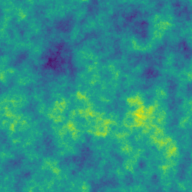
\includegraphics[scale=0.71]{random_field_matern_l_100_n_05-img0.png}
    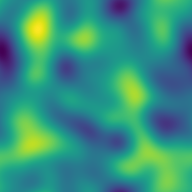
\includegraphics[scale=0.71]{random_field_matern_l_100_n_100-img0.png}
    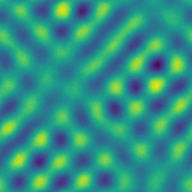
\includegraphics[scale=0.71]{random_field_cos_l_1000-img0.png}
    \caption{Samples drawn from random fields with three different covariance functions.}
    \label{fig:random_fields_intro.png}
\end{figure}








\subsection*{Gaussian Process Regression}
Say we now have a random process to model the structure of our optimization problem, more specifically a Gaussian process. It is characterized by a mean and covariance function quantifying the random structure. 
Possible realizations of such a process are shown in \cref{fig:sausage_plot_prior_matern}.
In Bayesian terms, this model is the prior, so the likelihood of samples before incorporating any measurement data.
How do we ensure, that the random process meets the measured values at the points of observation? 
For those points, how do we make it not random?
This is where the regression framework comes in. 
We can construct another random process, one that is an optimal predictor of the underlying process, conditional on the measured values.
It is constructed as a weighted linear combination of the measured values, with a covariance function that becomes zero at points of measurement. 
In Bayesian terms, this is the posterior.
In this way we can frame our beliefs as a prior distribution and update our model by conditioning on observations, thus arriving at a posterior distribution like \cref{fig:sausage_plot_posterior_matern}. 
This model is often referred to as a surrogate model.
One benefit of choosing Gaussian processes is that such a construction is then also a Gaussian process. 

% For a brief practical review of Bayesian statistics, we refer to~\cite{fornacon2022understanding}. \textcolor{red}{Maybe I leave out this last sentence.}

\begin{figure}[t]
    \centering
    %% Creator: Matplotlib, PGF backend
%%
%% To include the figure in your LaTeX document, write
%%   \input{<filename>.pgf}
%%
%% Make sure the required packages are loaded in your preamble
%%   \usepackage{pgf}
%%
%% Also ensure that all the required font packages are loaded; for instance,
%% the lmodern package is sometimes necessary when using math font.
%%   \usepackage{lmodern}
%%
%% Figures using additional raster images can only be included by \input if
%% they are in the same directory as the main LaTeX file. For loading figures
%% from other directories you can use the `import` package
%%   \usepackage{import}
%%
%% and then include the figures with
%%   \import{<path to file>}{<filename>.pgf}
%%
%% Matplotlib used the following preamble
%%   \def\mathdefault#1{#1}
%%   \everymath=\expandafter{\the\everymath\displaystyle}
%%   \usepackage[T1]{fontenc}
%%   \usepackage{siunitx}
%%   \usepackage{amssymb}
%%   \usepackage{amsmath}
%%   \makeatletter\@ifpackageloaded{underscore}{}{\usepackage[strings]{underscore}}\makeatother
%%
\begingroup%
\makeatletter%
\begin{pgfpicture}%
\pgfpathrectangle{\pgfpointorigin}{\pgfqpoint{5.788510in}{1.000000in}}%
\pgfusepath{use as bounding box, clip}%
\begin{pgfscope}%
\pgfsetbuttcap%
\pgfsetmiterjoin%
\definecolor{currentfill}{rgb}{1.000000,1.000000,1.000000}%
\pgfsetfillcolor{currentfill}%
\pgfsetlinewidth{0.000000pt}%
\definecolor{currentstroke}{rgb}{1.000000,1.000000,1.000000}%
\pgfsetstrokecolor{currentstroke}%
\pgfsetdash{}{0pt}%
\pgfpathmoveto{\pgfqpoint{0.000000in}{0.000000in}}%
\pgfpathlineto{\pgfqpoint{5.788510in}{0.000000in}}%
\pgfpathlineto{\pgfqpoint{5.788510in}{1.000000in}}%
\pgfpathlineto{\pgfqpoint{0.000000in}{1.000000in}}%
\pgfpathlineto{\pgfqpoint{0.000000in}{0.000000in}}%
\pgfpathclose%
\pgfusepath{fill}%
\end{pgfscope}%
\begin{pgfscope}%
\pgfsetbuttcap%
\pgfsetmiterjoin%
\definecolor{currentfill}{rgb}{1.000000,1.000000,1.000000}%
\pgfsetfillcolor{currentfill}%
\pgfsetlinewidth{0.000000pt}%
\definecolor{currentstroke}{rgb}{0.000000,0.000000,0.000000}%
\pgfsetstrokecolor{currentstroke}%
\pgfsetstrokeopacity{0.000000}%
\pgfsetdash{}{0pt}%
\pgfpathmoveto{\pgfqpoint{0.000000in}{0.000000in}}%
\pgfpathlineto{\pgfqpoint{5.788510in}{0.000000in}}%
\pgfpathlineto{\pgfqpoint{5.788510in}{0.800000in}}%
\pgfpathlineto{\pgfqpoint{0.000000in}{0.800000in}}%
\pgfpathlineto{\pgfqpoint{0.000000in}{0.000000in}}%
\pgfpathclose%
\pgfusepath{fill}%
\end{pgfscope}%
\begin{pgfscope}%
\pgfpathrectangle{\pgfqpoint{0.000000in}{0.000000in}}{\pgfqpoint{5.788510in}{0.800000in}}%
\pgfusepath{clip}%
\pgfsetbuttcap%
\pgfsetroundjoin%
\definecolor{currentfill}{rgb}{0.149020,0.274510,0.325490}%
\pgfsetfillcolor{currentfill}%
\pgfsetfillopacity{0.100000}%
\pgfsetlinewidth{1.003750pt}%
\definecolor{currentstroke}{rgb}{0.149020,0.274510,0.325490}%
\pgfsetstrokecolor{currentstroke}%
\pgfsetstrokeopacity{0.100000}%
\pgfsetdash{}{0pt}%
\pgfpathmoveto{\pgfqpoint{0.000000in}{0.723904in}}%
\pgfpathlineto{\pgfqpoint{0.000000in}{0.179224in}}%
\pgfpathlineto{\pgfqpoint{0.058470in}{0.179224in}}%
\pgfpathlineto{\pgfqpoint{0.116940in}{0.179224in}}%
\pgfpathlineto{\pgfqpoint{0.175409in}{0.179224in}}%
\pgfpathlineto{\pgfqpoint{0.233879in}{0.179224in}}%
\pgfpathlineto{\pgfqpoint{0.292349in}{0.179224in}}%
\pgfpathlineto{\pgfqpoint{0.350819in}{0.179224in}}%
\pgfpathlineto{\pgfqpoint{0.409289in}{0.179224in}}%
\pgfpathlineto{\pgfqpoint{0.467758in}{0.179224in}}%
\pgfpathlineto{\pgfqpoint{0.526228in}{0.179224in}}%
\pgfpathlineto{\pgfqpoint{0.584698in}{0.179224in}}%
\pgfpathlineto{\pgfqpoint{0.643168in}{0.179224in}}%
\pgfpathlineto{\pgfqpoint{0.701638in}{0.179224in}}%
\pgfpathlineto{\pgfqpoint{0.760107in}{0.179224in}}%
\pgfpathlineto{\pgfqpoint{0.818577in}{0.179224in}}%
\pgfpathlineto{\pgfqpoint{0.877047in}{0.179224in}}%
\pgfpathlineto{\pgfqpoint{0.935517in}{0.179224in}}%
\pgfpathlineto{\pgfqpoint{0.993987in}{0.179224in}}%
\pgfpathlineto{\pgfqpoint{1.052456in}{0.179224in}}%
\pgfpathlineto{\pgfqpoint{1.110926in}{0.179224in}}%
\pgfpathlineto{\pgfqpoint{1.169396in}{0.179224in}}%
\pgfpathlineto{\pgfqpoint{1.227866in}{0.179224in}}%
\pgfpathlineto{\pgfqpoint{1.286336in}{0.179224in}}%
\pgfpathlineto{\pgfqpoint{1.344805in}{0.179224in}}%
\pgfpathlineto{\pgfqpoint{1.403275in}{0.179224in}}%
\pgfpathlineto{\pgfqpoint{1.461745in}{0.179224in}}%
\pgfpathlineto{\pgfqpoint{1.520215in}{0.179224in}}%
\pgfpathlineto{\pgfqpoint{1.578685in}{0.179224in}}%
\pgfpathlineto{\pgfqpoint{1.637154in}{0.179224in}}%
\pgfpathlineto{\pgfqpoint{1.695624in}{0.179224in}}%
\pgfpathlineto{\pgfqpoint{1.754094in}{0.179224in}}%
\pgfpathlineto{\pgfqpoint{1.812564in}{0.179224in}}%
\pgfpathlineto{\pgfqpoint{1.871034in}{0.179224in}}%
\pgfpathlineto{\pgfqpoint{1.929503in}{0.179224in}}%
\pgfpathlineto{\pgfqpoint{1.987973in}{0.179224in}}%
\pgfpathlineto{\pgfqpoint{2.046443in}{0.179224in}}%
\pgfpathlineto{\pgfqpoint{2.104913in}{0.179224in}}%
\pgfpathlineto{\pgfqpoint{2.163383in}{0.179224in}}%
\pgfpathlineto{\pgfqpoint{2.221852in}{0.179224in}}%
\pgfpathlineto{\pgfqpoint{2.280322in}{0.179224in}}%
\pgfpathlineto{\pgfqpoint{2.338792in}{0.179224in}}%
\pgfpathlineto{\pgfqpoint{2.397262in}{0.179224in}}%
\pgfpathlineto{\pgfqpoint{2.455732in}{0.179224in}}%
\pgfpathlineto{\pgfqpoint{2.514201in}{0.179224in}}%
\pgfpathlineto{\pgfqpoint{2.572671in}{0.179224in}}%
\pgfpathlineto{\pgfqpoint{2.631141in}{0.179224in}}%
\pgfpathlineto{\pgfqpoint{2.689611in}{0.179224in}}%
\pgfpathlineto{\pgfqpoint{2.748081in}{0.179224in}}%
\pgfpathlineto{\pgfqpoint{2.806550in}{0.179224in}}%
\pgfpathlineto{\pgfqpoint{2.865020in}{0.179224in}}%
\pgfpathlineto{\pgfqpoint{2.923490in}{0.179224in}}%
\pgfpathlineto{\pgfqpoint{2.981960in}{0.179224in}}%
\pgfpathlineto{\pgfqpoint{3.040429in}{0.179224in}}%
\pgfpathlineto{\pgfqpoint{3.098899in}{0.179224in}}%
\pgfpathlineto{\pgfqpoint{3.157369in}{0.179224in}}%
\pgfpathlineto{\pgfqpoint{3.215839in}{0.179224in}}%
\pgfpathlineto{\pgfqpoint{3.274309in}{0.179224in}}%
\pgfpathlineto{\pgfqpoint{3.332778in}{0.179224in}}%
\pgfpathlineto{\pgfqpoint{3.391248in}{0.179224in}}%
\pgfpathlineto{\pgfqpoint{3.449718in}{0.179224in}}%
\pgfpathlineto{\pgfqpoint{3.508188in}{0.179224in}}%
\pgfpathlineto{\pgfqpoint{3.566658in}{0.179224in}}%
\pgfpathlineto{\pgfqpoint{3.625127in}{0.179224in}}%
\pgfpathlineto{\pgfqpoint{3.683597in}{0.179224in}}%
\pgfpathlineto{\pgfqpoint{3.742067in}{0.179224in}}%
\pgfpathlineto{\pgfqpoint{3.800537in}{0.179224in}}%
\pgfpathlineto{\pgfqpoint{3.859007in}{0.179224in}}%
\pgfpathlineto{\pgfqpoint{3.917476in}{0.179224in}}%
\pgfpathlineto{\pgfqpoint{3.975946in}{0.179224in}}%
\pgfpathlineto{\pgfqpoint{4.034416in}{0.179224in}}%
\pgfpathlineto{\pgfqpoint{4.092886in}{0.179224in}}%
\pgfpathlineto{\pgfqpoint{4.151356in}{0.179224in}}%
\pgfpathlineto{\pgfqpoint{4.209825in}{0.179224in}}%
\pgfpathlineto{\pgfqpoint{4.268295in}{0.179224in}}%
\pgfpathlineto{\pgfqpoint{4.326765in}{0.179224in}}%
\pgfpathlineto{\pgfqpoint{4.385235in}{0.179224in}}%
\pgfpathlineto{\pgfqpoint{4.443705in}{0.179224in}}%
\pgfpathlineto{\pgfqpoint{4.502174in}{0.179224in}}%
\pgfpathlineto{\pgfqpoint{4.560644in}{0.179224in}}%
\pgfpathlineto{\pgfqpoint{4.619114in}{0.179224in}}%
\pgfpathlineto{\pgfqpoint{4.677584in}{0.179224in}}%
\pgfpathlineto{\pgfqpoint{4.736054in}{0.179224in}}%
\pgfpathlineto{\pgfqpoint{4.794523in}{0.179224in}}%
\pgfpathlineto{\pgfqpoint{4.852993in}{0.179224in}}%
\pgfpathlineto{\pgfqpoint{4.911463in}{0.179224in}}%
\pgfpathlineto{\pgfqpoint{4.969933in}{0.179224in}}%
\pgfpathlineto{\pgfqpoint{5.028403in}{0.179224in}}%
\pgfpathlineto{\pgfqpoint{5.086872in}{0.179224in}}%
\pgfpathlineto{\pgfqpoint{5.145342in}{0.179224in}}%
\pgfpathlineto{\pgfqpoint{5.203812in}{0.179224in}}%
\pgfpathlineto{\pgfqpoint{5.262282in}{0.179224in}}%
\pgfpathlineto{\pgfqpoint{5.320752in}{0.179224in}}%
\pgfpathlineto{\pgfqpoint{5.379221in}{0.179224in}}%
\pgfpathlineto{\pgfqpoint{5.437691in}{0.179224in}}%
\pgfpathlineto{\pgfqpoint{5.496161in}{0.179224in}}%
\pgfpathlineto{\pgfqpoint{5.554631in}{0.179224in}}%
\pgfpathlineto{\pgfqpoint{5.613101in}{0.179224in}}%
\pgfpathlineto{\pgfqpoint{5.671570in}{0.179224in}}%
\pgfpathlineto{\pgfqpoint{5.730040in}{0.179224in}}%
\pgfpathlineto{\pgfqpoint{5.788510in}{0.179224in}}%
\pgfpathlineto{\pgfqpoint{5.788510in}{0.723904in}}%
\pgfpathlineto{\pgfqpoint{5.788510in}{0.723904in}}%
\pgfpathlineto{\pgfqpoint{5.730040in}{0.723904in}}%
\pgfpathlineto{\pgfqpoint{5.671570in}{0.723904in}}%
\pgfpathlineto{\pgfqpoint{5.613101in}{0.723904in}}%
\pgfpathlineto{\pgfqpoint{5.554631in}{0.723904in}}%
\pgfpathlineto{\pgfqpoint{5.496161in}{0.723904in}}%
\pgfpathlineto{\pgfqpoint{5.437691in}{0.723904in}}%
\pgfpathlineto{\pgfqpoint{5.379221in}{0.723904in}}%
\pgfpathlineto{\pgfqpoint{5.320752in}{0.723904in}}%
\pgfpathlineto{\pgfqpoint{5.262282in}{0.723904in}}%
\pgfpathlineto{\pgfqpoint{5.203812in}{0.723904in}}%
\pgfpathlineto{\pgfqpoint{5.145342in}{0.723904in}}%
\pgfpathlineto{\pgfqpoint{5.086872in}{0.723904in}}%
\pgfpathlineto{\pgfqpoint{5.028403in}{0.723904in}}%
\pgfpathlineto{\pgfqpoint{4.969933in}{0.723904in}}%
\pgfpathlineto{\pgfqpoint{4.911463in}{0.723904in}}%
\pgfpathlineto{\pgfqpoint{4.852993in}{0.723904in}}%
\pgfpathlineto{\pgfqpoint{4.794523in}{0.723904in}}%
\pgfpathlineto{\pgfqpoint{4.736054in}{0.723904in}}%
\pgfpathlineto{\pgfqpoint{4.677584in}{0.723904in}}%
\pgfpathlineto{\pgfqpoint{4.619114in}{0.723904in}}%
\pgfpathlineto{\pgfqpoint{4.560644in}{0.723904in}}%
\pgfpathlineto{\pgfqpoint{4.502174in}{0.723904in}}%
\pgfpathlineto{\pgfqpoint{4.443705in}{0.723904in}}%
\pgfpathlineto{\pgfqpoint{4.385235in}{0.723904in}}%
\pgfpathlineto{\pgfqpoint{4.326765in}{0.723904in}}%
\pgfpathlineto{\pgfqpoint{4.268295in}{0.723904in}}%
\pgfpathlineto{\pgfqpoint{4.209825in}{0.723904in}}%
\pgfpathlineto{\pgfqpoint{4.151356in}{0.723904in}}%
\pgfpathlineto{\pgfqpoint{4.092886in}{0.723904in}}%
\pgfpathlineto{\pgfqpoint{4.034416in}{0.723904in}}%
\pgfpathlineto{\pgfqpoint{3.975946in}{0.723904in}}%
\pgfpathlineto{\pgfqpoint{3.917476in}{0.723904in}}%
\pgfpathlineto{\pgfqpoint{3.859007in}{0.723904in}}%
\pgfpathlineto{\pgfqpoint{3.800537in}{0.723904in}}%
\pgfpathlineto{\pgfqpoint{3.742067in}{0.723904in}}%
\pgfpathlineto{\pgfqpoint{3.683597in}{0.723904in}}%
\pgfpathlineto{\pgfqpoint{3.625127in}{0.723904in}}%
\pgfpathlineto{\pgfqpoint{3.566658in}{0.723904in}}%
\pgfpathlineto{\pgfqpoint{3.508188in}{0.723904in}}%
\pgfpathlineto{\pgfqpoint{3.449718in}{0.723904in}}%
\pgfpathlineto{\pgfqpoint{3.391248in}{0.723904in}}%
\pgfpathlineto{\pgfqpoint{3.332778in}{0.723904in}}%
\pgfpathlineto{\pgfqpoint{3.274309in}{0.723904in}}%
\pgfpathlineto{\pgfqpoint{3.215839in}{0.723904in}}%
\pgfpathlineto{\pgfqpoint{3.157369in}{0.723904in}}%
\pgfpathlineto{\pgfqpoint{3.098899in}{0.723904in}}%
\pgfpathlineto{\pgfqpoint{3.040429in}{0.723904in}}%
\pgfpathlineto{\pgfqpoint{2.981960in}{0.723904in}}%
\pgfpathlineto{\pgfqpoint{2.923490in}{0.723904in}}%
\pgfpathlineto{\pgfqpoint{2.865020in}{0.723904in}}%
\pgfpathlineto{\pgfqpoint{2.806550in}{0.723904in}}%
\pgfpathlineto{\pgfqpoint{2.748081in}{0.723904in}}%
\pgfpathlineto{\pgfqpoint{2.689611in}{0.723904in}}%
\pgfpathlineto{\pgfqpoint{2.631141in}{0.723904in}}%
\pgfpathlineto{\pgfqpoint{2.572671in}{0.723904in}}%
\pgfpathlineto{\pgfqpoint{2.514201in}{0.723904in}}%
\pgfpathlineto{\pgfqpoint{2.455732in}{0.723904in}}%
\pgfpathlineto{\pgfqpoint{2.397262in}{0.723904in}}%
\pgfpathlineto{\pgfqpoint{2.338792in}{0.723904in}}%
\pgfpathlineto{\pgfqpoint{2.280322in}{0.723904in}}%
\pgfpathlineto{\pgfqpoint{2.221852in}{0.723904in}}%
\pgfpathlineto{\pgfqpoint{2.163383in}{0.723904in}}%
\pgfpathlineto{\pgfqpoint{2.104913in}{0.723904in}}%
\pgfpathlineto{\pgfqpoint{2.046443in}{0.723904in}}%
\pgfpathlineto{\pgfqpoint{1.987973in}{0.723904in}}%
\pgfpathlineto{\pgfqpoint{1.929503in}{0.723904in}}%
\pgfpathlineto{\pgfqpoint{1.871034in}{0.723904in}}%
\pgfpathlineto{\pgfqpoint{1.812564in}{0.723904in}}%
\pgfpathlineto{\pgfqpoint{1.754094in}{0.723904in}}%
\pgfpathlineto{\pgfqpoint{1.695624in}{0.723904in}}%
\pgfpathlineto{\pgfqpoint{1.637154in}{0.723904in}}%
\pgfpathlineto{\pgfqpoint{1.578685in}{0.723904in}}%
\pgfpathlineto{\pgfqpoint{1.520215in}{0.723904in}}%
\pgfpathlineto{\pgfqpoint{1.461745in}{0.723904in}}%
\pgfpathlineto{\pgfqpoint{1.403275in}{0.723904in}}%
\pgfpathlineto{\pgfqpoint{1.344805in}{0.723904in}}%
\pgfpathlineto{\pgfqpoint{1.286336in}{0.723904in}}%
\pgfpathlineto{\pgfqpoint{1.227866in}{0.723904in}}%
\pgfpathlineto{\pgfqpoint{1.169396in}{0.723904in}}%
\pgfpathlineto{\pgfqpoint{1.110926in}{0.723904in}}%
\pgfpathlineto{\pgfqpoint{1.052456in}{0.723904in}}%
\pgfpathlineto{\pgfqpoint{0.993987in}{0.723904in}}%
\pgfpathlineto{\pgfqpoint{0.935517in}{0.723904in}}%
\pgfpathlineto{\pgfqpoint{0.877047in}{0.723904in}}%
\pgfpathlineto{\pgfqpoint{0.818577in}{0.723904in}}%
\pgfpathlineto{\pgfqpoint{0.760107in}{0.723904in}}%
\pgfpathlineto{\pgfqpoint{0.701638in}{0.723904in}}%
\pgfpathlineto{\pgfqpoint{0.643168in}{0.723904in}}%
\pgfpathlineto{\pgfqpoint{0.584698in}{0.723904in}}%
\pgfpathlineto{\pgfqpoint{0.526228in}{0.723904in}}%
\pgfpathlineto{\pgfqpoint{0.467758in}{0.723904in}}%
\pgfpathlineto{\pgfqpoint{0.409289in}{0.723904in}}%
\pgfpathlineto{\pgfqpoint{0.350819in}{0.723904in}}%
\pgfpathlineto{\pgfqpoint{0.292349in}{0.723904in}}%
\pgfpathlineto{\pgfqpoint{0.233879in}{0.723904in}}%
\pgfpathlineto{\pgfqpoint{0.175409in}{0.723904in}}%
\pgfpathlineto{\pgfqpoint{0.116940in}{0.723904in}}%
\pgfpathlineto{\pgfqpoint{0.058470in}{0.723904in}}%
\pgfpathlineto{\pgfqpoint{0.000000in}{0.723904in}}%
\pgfpathlineto{\pgfqpoint{0.000000in}{0.723904in}}%
\pgfpathclose%
\pgfusepath{stroke,fill}%
\end{pgfscope}%
\begin{pgfscope}%
\pgfpathrectangle{\pgfqpoint{0.000000in}{0.000000in}}{\pgfqpoint{5.788510in}{0.800000in}}%
\pgfusepath{clip}%
\pgfsetrectcap%
\pgfsetroundjoin%
\pgfsetlinewidth{1.505625pt}%
\definecolor{currentstroke}{rgb}{1.000000,0.745098,0.043137}%
\pgfsetstrokecolor{currentstroke}%
\pgfsetdash{}{0pt}%
\pgfpathmoveto{\pgfqpoint{0.000000in}{0.036364in}}%
\pgfpathlineto{\pgfqpoint{0.058470in}{0.039774in}}%
\pgfpathlineto{\pgfqpoint{0.116940in}{0.044612in}}%
\pgfpathlineto{\pgfqpoint{0.175409in}{0.050882in}}%
\pgfpathlineto{\pgfqpoint{0.233879in}{0.058570in}}%
\pgfpathlineto{\pgfqpoint{0.292349in}{0.067642in}}%
\pgfpathlineto{\pgfqpoint{0.350819in}{0.078044in}}%
\pgfpathlineto{\pgfqpoint{0.409289in}{0.089702in}}%
\pgfpathlineto{\pgfqpoint{0.467758in}{0.102524in}}%
\pgfpathlineto{\pgfqpoint{0.526228in}{0.116399in}}%
\pgfpathlineto{\pgfqpoint{0.584698in}{0.131199in}}%
\pgfpathlineto{\pgfqpoint{0.643168in}{0.146784in}}%
\pgfpathlineto{\pgfqpoint{0.701638in}{0.162998in}}%
\pgfpathlineto{\pgfqpoint{0.760107in}{0.179678in}}%
\pgfpathlineto{\pgfqpoint{0.818577in}{0.196651in}}%
\pgfpathlineto{\pgfqpoint{0.877047in}{0.213741in}}%
\pgfpathlineto{\pgfqpoint{0.935517in}{0.230768in}}%
\pgfpathlineto{\pgfqpoint{0.993987in}{0.247556in}}%
\pgfpathlineto{\pgfqpoint{1.052456in}{0.263931in}}%
\pgfpathlineto{\pgfqpoint{1.110926in}{0.279725in}}%
\pgfpathlineto{\pgfqpoint{1.169396in}{0.294779in}}%
\pgfpathlineto{\pgfqpoint{1.227866in}{0.308948in}}%
\pgfpathlineto{\pgfqpoint{1.286336in}{0.322096in}}%
\pgfpathlineto{\pgfqpoint{1.344805in}{0.334106in}}%
\pgfpathlineto{\pgfqpoint{1.403275in}{0.344875in}}%
\pgfpathlineto{\pgfqpoint{1.461745in}{0.354320in}}%
\pgfpathlineto{\pgfqpoint{1.520215in}{0.362374in}}%
\pgfpathlineto{\pgfqpoint{1.578685in}{0.368991in}}%
\pgfpathlineto{\pgfqpoint{1.637154in}{0.374144in}}%
\pgfpathlineto{\pgfqpoint{1.695624in}{0.377825in}}%
\pgfpathlineto{\pgfqpoint{1.754094in}{0.380046in}}%
\pgfpathlineto{\pgfqpoint{1.812564in}{0.380836in}}%
\pgfpathlineto{\pgfqpoint{1.871034in}{0.380242in}}%
\pgfpathlineto{\pgfqpoint{1.929503in}{0.378329in}}%
\pgfpathlineto{\pgfqpoint{1.987973in}{0.375175in}}%
\pgfpathlineto{\pgfqpoint{2.046443in}{0.370875in}}%
\pgfpathlineto{\pgfqpoint{2.104913in}{0.365533in}}%
\pgfpathlineto{\pgfqpoint{2.163383in}{0.359268in}}%
\pgfpathlineto{\pgfqpoint{2.221852in}{0.352205in}}%
\pgfpathlineto{\pgfqpoint{2.280322in}{0.344476in}}%
\pgfpathlineto{\pgfqpoint{2.338792in}{0.336219in}}%
\pgfpathlineto{\pgfqpoint{2.397262in}{0.327576in}}%
\pgfpathlineto{\pgfqpoint{2.455732in}{0.318687in}}%
\pgfpathlineto{\pgfqpoint{2.514201in}{0.309693in}}%
\pgfpathlineto{\pgfqpoint{2.572671in}{0.300731in}}%
\pgfpathlineto{\pgfqpoint{2.631141in}{0.291930in}}%
\pgfpathlineto{\pgfqpoint{2.689611in}{0.283416in}}%
\pgfpathlineto{\pgfqpoint{2.748081in}{0.275301in}}%
\pgfpathlineto{\pgfqpoint{2.806550in}{0.267688in}}%
\pgfpathlineto{\pgfqpoint{2.865020in}{0.260667in}}%
\pgfpathlineto{\pgfqpoint{2.923490in}{0.254315in}}%
\pgfpathlineto{\pgfqpoint{2.981960in}{0.248692in}}%
\pgfpathlineto{\pgfqpoint{3.040429in}{0.243846in}}%
\pgfpathlineto{\pgfqpoint{3.098899in}{0.239806in}}%
\pgfpathlineto{\pgfqpoint{3.157369in}{0.236589in}}%
\pgfpathlineto{\pgfqpoint{3.215839in}{0.234193in}}%
\pgfpathlineto{\pgfqpoint{3.274309in}{0.232606in}}%
\pgfpathlineto{\pgfqpoint{3.332778in}{0.231800in}}%
\pgfpathlineto{\pgfqpoint{3.391248in}{0.231737in}}%
\pgfpathlineto{\pgfqpoint{3.449718in}{0.232367in}}%
\pgfpathlineto{\pgfqpoint{3.508188in}{0.233635in}}%
\pgfpathlineto{\pgfqpoint{3.566658in}{0.235478in}}%
\pgfpathlineto{\pgfqpoint{3.625127in}{0.237828in}}%
\pgfpathlineto{\pgfqpoint{3.683597in}{0.240618in}}%
\pgfpathlineto{\pgfqpoint{3.742067in}{0.243777in}}%
\pgfpathlineto{\pgfqpoint{3.800537in}{0.247240in}}%
\pgfpathlineto{\pgfqpoint{3.859007in}{0.250945in}}%
\pgfpathlineto{\pgfqpoint{3.917476in}{0.254832in}}%
\pgfpathlineto{\pgfqpoint{3.975946in}{0.258852in}}%
\pgfpathlineto{\pgfqpoint{4.034416in}{0.262961in}}%
\pgfpathlineto{\pgfqpoint{4.092886in}{0.267124in}}%
\pgfpathlineto{\pgfqpoint{4.151356in}{0.271316in}}%
\pgfpathlineto{\pgfqpoint{4.209825in}{0.275518in}}%
\pgfpathlineto{\pgfqpoint{4.268295in}{0.279724in}}%
\pgfpathlineto{\pgfqpoint{4.326765in}{0.283931in}}%
\pgfpathlineto{\pgfqpoint{4.385235in}{0.288147in}}%
\pgfpathlineto{\pgfqpoint{4.443705in}{0.292386in}}%
\pgfpathlineto{\pgfqpoint{4.502174in}{0.296664in}}%
\pgfpathlineto{\pgfqpoint{4.560644in}{0.301005in}}%
\pgfpathlineto{\pgfqpoint{4.619114in}{0.305434in}}%
\pgfpathlineto{\pgfqpoint{4.677584in}{0.309976in}}%
\pgfpathlineto{\pgfqpoint{4.736054in}{0.314658in}}%
\pgfpathlineto{\pgfqpoint{4.794523in}{0.319504in}}%
\pgfpathlineto{\pgfqpoint{4.852993in}{0.324537in}}%
\pgfpathlineto{\pgfqpoint{4.911463in}{0.329775in}}%
\pgfpathlineto{\pgfqpoint{4.969933in}{0.335233in}}%
\pgfpathlineto{\pgfqpoint{5.028403in}{0.340919in}}%
\pgfpathlineto{\pgfqpoint{5.086872in}{0.346838in}}%
\pgfpathlineto{\pgfqpoint{5.145342in}{0.352988in}}%
\pgfpathlineto{\pgfqpoint{5.203812in}{0.359361in}}%
\pgfpathlineto{\pgfqpoint{5.262282in}{0.365945in}}%
\pgfpathlineto{\pgfqpoint{5.320752in}{0.372722in}}%
\pgfpathlineto{\pgfqpoint{5.379221in}{0.379667in}}%
\pgfpathlineto{\pgfqpoint{5.437691in}{0.386753in}}%
\pgfpathlineto{\pgfqpoint{5.496161in}{0.393948in}}%
\pgfpathlineto{\pgfqpoint{5.554631in}{0.401219in}}%
\pgfpathlineto{\pgfqpoint{5.613101in}{0.408527in}}%
\pgfpathlineto{\pgfqpoint{5.671570in}{0.415833in}}%
\pgfpathlineto{\pgfqpoint{5.730040in}{0.423098in}}%
\pgfpathlineto{\pgfqpoint{5.788510in}{0.430280in}}%
\pgfusepath{stroke}%
\end{pgfscope}%
\begin{pgfscope}%
\pgfpathrectangle{\pgfqpoint{0.000000in}{0.000000in}}{\pgfqpoint{5.788510in}{0.800000in}}%
\pgfusepath{clip}%
\pgfsetrectcap%
\pgfsetroundjoin%
\pgfsetlinewidth{1.505625pt}%
\definecolor{currentstroke}{rgb}{0.984314,0.337255,0.027451}%
\pgfsetstrokecolor{currentstroke}%
\pgfsetdash{}{0pt}%
\pgfpathmoveto{\pgfqpoint{0.000000in}{0.600210in}}%
\pgfpathlineto{\pgfqpoint{0.058470in}{0.592034in}}%
\pgfpathlineto{\pgfqpoint{0.116940in}{0.583564in}}%
\pgfpathlineto{\pgfqpoint{0.175409in}{0.574849in}}%
\pgfpathlineto{\pgfqpoint{0.233879in}{0.565941in}}%
\pgfpathlineto{\pgfqpoint{0.292349in}{0.556891in}}%
\pgfpathlineto{\pgfqpoint{0.350819in}{0.547748in}}%
\pgfpathlineto{\pgfqpoint{0.409289in}{0.538562in}}%
\pgfpathlineto{\pgfqpoint{0.467758in}{0.529378in}}%
\pgfpathlineto{\pgfqpoint{0.526228in}{0.520241in}}%
\pgfpathlineto{\pgfqpoint{0.584698in}{0.511189in}}%
\pgfpathlineto{\pgfqpoint{0.643168in}{0.502260in}}%
\pgfpathlineto{\pgfqpoint{0.701638in}{0.493487in}}%
\pgfpathlineto{\pgfqpoint{0.760107in}{0.484899in}}%
\pgfpathlineto{\pgfqpoint{0.818577in}{0.476520in}}%
\pgfpathlineto{\pgfqpoint{0.877047in}{0.468374in}}%
\pgfpathlineto{\pgfqpoint{0.935517in}{0.460478in}}%
\pgfpathlineto{\pgfqpoint{0.993987in}{0.452846in}}%
\pgfpathlineto{\pgfqpoint{1.052456in}{0.445489in}}%
\pgfpathlineto{\pgfqpoint{1.110926in}{0.438413in}}%
\pgfpathlineto{\pgfqpoint{1.169396in}{0.431622in}}%
\pgfpathlineto{\pgfqpoint{1.227866in}{0.425114in}}%
\pgfpathlineto{\pgfqpoint{1.286336in}{0.418882in}}%
\pgfpathlineto{\pgfqpoint{1.344805in}{0.412914in}}%
\pgfpathlineto{\pgfqpoint{1.403275in}{0.407193in}}%
\pgfpathlineto{\pgfqpoint{1.461745in}{0.401693in}}%
\pgfpathlineto{\pgfqpoint{1.520215in}{0.396383in}}%
\pgfpathlineto{\pgfqpoint{1.578685in}{0.391224in}}%
\pgfpathlineto{\pgfqpoint{1.637154in}{0.386167in}}%
\pgfpathlineto{\pgfqpoint{1.695624in}{0.381157in}}%
\pgfpathlineto{\pgfqpoint{1.754094in}{0.376131in}}%
\pgfpathlineto{\pgfqpoint{1.812564in}{0.371018in}}%
\pgfpathlineto{\pgfqpoint{1.871034in}{0.365740in}}%
\pgfpathlineto{\pgfqpoint{1.929503in}{0.360216in}}%
\pgfpathlineto{\pgfqpoint{1.987973in}{0.354359in}}%
\pgfpathlineto{\pgfqpoint{2.046443in}{0.348082in}}%
\pgfpathlineto{\pgfqpoint{2.104913in}{0.341300in}}%
\pgfpathlineto{\pgfqpoint{2.163383in}{0.333931in}}%
\pgfpathlineto{\pgfqpoint{2.221852in}{0.325900in}}%
\pgfpathlineto{\pgfqpoint{2.280322in}{0.317142in}}%
\pgfpathlineto{\pgfqpoint{2.338792in}{0.307606in}}%
\pgfpathlineto{\pgfqpoint{2.397262in}{0.297254in}}%
\pgfpathlineto{\pgfqpoint{2.455732in}{0.286070in}}%
\pgfpathlineto{\pgfqpoint{2.514201in}{0.274058in}}%
\pgfpathlineto{\pgfqpoint{2.572671in}{0.261243in}}%
\pgfpathlineto{\pgfqpoint{2.631141in}{0.247676in}}%
\pgfpathlineto{\pgfqpoint{2.689611in}{0.233431in}}%
\pgfpathlineto{\pgfqpoint{2.748081in}{0.218607in}}%
\pgfpathlineto{\pgfqpoint{2.806550in}{0.203326in}}%
\pgfpathlineto{\pgfqpoint{2.865020in}{0.187731in}}%
\pgfpathlineto{\pgfqpoint{2.923490in}{0.171986in}}%
\pgfpathlineto{\pgfqpoint{2.981960in}{0.156269in}}%
\pgfpathlineto{\pgfqpoint{3.040429in}{0.140770in}}%
\pgfpathlineto{\pgfqpoint{3.098899in}{0.125689in}}%
\pgfpathlineto{\pgfqpoint{3.157369in}{0.111228in}}%
\pgfpathlineto{\pgfqpoint{3.215839in}{0.097588in}}%
\pgfpathlineto{\pgfqpoint{3.274309in}{0.084964in}}%
\pgfpathlineto{\pgfqpoint{3.332778in}{0.073540in}}%
\pgfpathlineto{\pgfqpoint{3.391248in}{0.063485in}}%
\pgfpathlineto{\pgfqpoint{3.449718in}{0.054950in}}%
\pgfpathlineto{\pgfqpoint{3.508188in}{0.048062in}}%
\pgfpathlineto{\pgfqpoint{3.566658in}{0.042922in}}%
\pgfpathlineto{\pgfqpoint{3.625127in}{0.039605in}}%
\pgfpathlineto{\pgfqpoint{3.683597in}{0.038157in}}%
\pgfpathlineto{\pgfqpoint{3.742067in}{0.038593in}}%
\pgfpathlineto{\pgfqpoint{3.800537in}{0.040901in}}%
\pgfpathlineto{\pgfqpoint{3.859007in}{0.045039in}}%
\pgfpathlineto{\pgfqpoint{3.917476in}{0.050939in}}%
\pgfpathlineto{\pgfqpoint{3.975946in}{0.058509in}}%
\pgfpathlineto{\pgfqpoint{4.034416in}{0.067636in}}%
\pgfpathlineto{\pgfqpoint{4.092886in}{0.078189in}}%
\pgfpathlineto{\pgfqpoint{4.151356in}{0.090022in}}%
\pgfpathlineto{\pgfqpoint{4.209825in}{0.102979in}}%
\pgfpathlineto{\pgfqpoint{4.268295in}{0.116895in}}%
\pgfpathlineto{\pgfqpoint{4.326765in}{0.131606in}}%
\pgfpathlineto{\pgfqpoint{4.385235in}{0.146943in}}%
\pgfpathlineto{\pgfqpoint{4.443705in}{0.162743in}}%
\pgfpathlineto{\pgfqpoint{4.502174in}{0.178849in}}%
\pgfpathlineto{\pgfqpoint{4.560644in}{0.195112in}}%
\pgfpathlineto{\pgfqpoint{4.619114in}{0.211395in}}%
\pgfpathlineto{\pgfqpoint{4.677584in}{0.227572in}}%
\pgfpathlineto{\pgfqpoint{4.736054in}{0.243529in}}%
\pgfpathlineto{\pgfqpoint{4.794523in}{0.259167in}}%
\pgfpathlineto{\pgfqpoint{4.852993in}{0.274402in}}%
\pgfpathlineto{\pgfqpoint{4.911463in}{0.289162in}}%
\pgfpathlineto{\pgfqpoint{4.969933in}{0.303389in}}%
\pgfpathlineto{\pgfqpoint{5.028403in}{0.317036in}}%
\pgfpathlineto{\pgfqpoint{5.086872in}{0.330068in}}%
\pgfpathlineto{\pgfqpoint{5.145342in}{0.342461in}}%
\pgfpathlineto{\pgfqpoint{5.203812in}{0.354199in}}%
\pgfpathlineto{\pgfqpoint{5.262282in}{0.365271in}}%
\pgfpathlineto{\pgfqpoint{5.320752in}{0.375674in}}%
\pgfpathlineto{\pgfqpoint{5.379221in}{0.385410in}}%
\pgfpathlineto{\pgfqpoint{5.437691in}{0.394483in}}%
\pgfpathlineto{\pgfqpoint{5.496161in}{0.402897in}}%
\pgfpathlineto{\pgfqpoint{5.554631in}{0.410660in}}%
\pgfpathlineto{\pgfqpoint{5.613101in}{0.417780in}}%
\pgfpathlineto{\pgfqpoint{5.671570in}{0.424260in}}%
\pgfpathlineto{\pgfqpoint{5.730040in}{0.430107in}}%
\pgfpathlineto{\pgfqpoint{5.788510in}{0.435323in}}%
\pgfusepath{stroke}%
\end{pgfscope}%
\begin{pgfscope}%
\pgfpathrectangle{\pgfqpoint{0.000000in}{0.000000in}}{\pgfqpoint{5.788510in}{0.800000in}}%
\pgfusepath{clip}%
\pgfsetrectcap%
\pgfsetroundjoin%
\pgfsetlinewidth{1.505625pt}%
\definecolor{currentstroke}{rgb}{1.000000,0.000000,0.431373}%
\pgfsetstrokecolor{currentstroke}%
\pgfsetdash{}{0pt}%
\pgfpathmoveto{\pgfqpoint{0.000000in}{0.281863in}}%
\pgfpathlineto{\pgfqpoint{0.058470in}{0.292083in}}%
\pgfpathlineto{\pgfqpoint{0.116940in}{0.302754in}}%
\pgfpathlineto{\pgfqpoint{0.175409in}{0.313836in}}%
\pgfpathlineto{\pgfqpoint{0.233879in}{0.325276in}}%
\pgfpathlineto{\pgfqpoint{0.292349in}{0.337019in}}%
\pgfpathlineto{\pgfqpoint{0.350819in}{0.349001in}}%
\pgfpathlineto{\pgfqpoint{0.409289in}{0.361152in}}%
\pgfpathlineto{\pgfqpoint{0.467758in}{0.373400in}}%
\pgfpathlineto{\pgfqpoint{0.526228in}{0.385668in}}%
\pgfpathlineto{\pgfqpoint{0.584698in}{0.397879in}}%
\pgfpathlineto{\pgfqpoint{0.643168in}{0.409955in}}%
\pgfpathlineto{\pgfqpoint{0.701638in}{0.421820in}}%
\pgfpathlineto{\pgfqpoint{0.760107in}{0.433401in}}%
\pgfpathlineto{\pgfqpoint{0.818577in}{0.444628in}}%
\pgfpathlineto{\pgfqpoint{0.877047in}{0.455439in}}%
\pgfpathlineto{\pgfqpoint{0.935517in}{0.465776in}}%
\pgfpathlineto{\pgfqpoint{0.993987in}{0.475590in}}%
\pgfpathlineto{\pgfqpoint{1.052456in}{0.484840in}}%
\pgfpathlineto{\pgfqpoint{1.110926in}{0.493494in}}%
\pgfpathlineto{\pgfqpoint{1.169396in}{0.501530in}}%
\pgfpathlineto{\pgfqpoint{1.227866in}{0.508933in}}%
\pgfpathlineto{\pgfqpoint{1.286336in}{0.515700in}}%
\pgfpathlineto{\pgfqpoint{1.344805in}{0.521836in}}%
\pgfpathlineto{\pgfqpoint{1.403275in}{0.527352in}}%
\pgfpathlineto{\pgfqpoint{1.461745in}{0.532270in}}%
\pgfpathlineto{\pgfqpoint{1.520215in}{0.536618in}}%
\pgfpathlineto{\pgfqpoint{1.578685in}{0.540426in}}%
\pgfpathlineto{\pgfqpoint{1.637154in}{0.543734in}}%
\pgfpathlineto{\pgfqpoint{1.695624in}{0.546581in}}%
\pgfpathlineto{\pgfqpoint{1.754094in}{0.549010in}}%
\pgfpathlineto{\pgfqpoint{1.812564in}{0.551065in}}%
\pgfpathlineto{\pgfqpoint{1.871034in}{0.552789in}}%
\pgfpathlineto{\pgfqpoint{1.929503in}{0.554223in}}%
\pgfpathlineto{\pgfqpoint{1.987973in}{0.555407in}}%
\pgfpathlineto{\pgfqpoint{2.046443in}{0.556376in}}%
\pgfpathlineto{\pgfqpoint{2.104913in}{0.557163in}}%
\pgfpathlineto{\pgfqpoint{2.163383in}{0.557794in}}%
\pgfpathlineto{\pgfqpoint{2.221852in}{0.558292in}}%
\pgfpathlineto{\pgfqpoint{2.280322in}{0.558671in}}%
\pgfpathlineto{\pgfqpoint{2.338792in}{0.558945in}}%
\pgfpathlineto{\pgfqpoint{2.397262in}{0.559116in}}%
\pgfpathlineto{\pgfqpoint{2.455732in}{0.559187in}}%
\pgfpathlineto{\pgfqpoint{2.514201in}{0.559152in}}%
\pgfpathlineto{\pgfqpoint{2.572671in}{0.559001in}}%
\pgfpathlineto{\pgfqpoint{2.631141in}{0.558722in}}%
\pgfpathlineto{\pgfqpoint{2.689611in}{0.558297in}}%
\pgfpathlineto{\pgfqpoint{2.748081in}{0.557708in}}%
\pgfpathlineto{\pgfqpoint{2.806550in}{0.556932in}}%
\pgfpathlineto{\pgfqpoint{2.865020in}{0.555949in}}%
\pgfpathlineto{\pgfqpoint{2.923490in}{0.554733in}}%
\pgfpathlineto{\pgfqpoint{2.981960in}{0.553263in}}%
\pgfpathlineto{\pgfqpoint{3.040429in}{0.551516in}}%
\pgfpathlineto{\pgfqpoint{3.098899in}{0.549469in}}%
\pgfpathlineto{\pgfqpoint{3.157369in}{0.547105in}}%
\pgfpathlineto{\pgfqpoint{3.215839in}{0.544405in}}%
\pgfpathlineto{\pgfqpoint{3.274309in}{0.541355in}}%
\pgfpathlineto{\pgfqpoint{3.332778in}{0.537944in}}%
\pgfpathlineto{\pgfqpoint{3.391248in}{0.534163in}}%
\pgfpathlineto{\pgfqpoint{3.449718in}{0.530008in}}%
\pgfpathlineto{\pgfqpoint{3.508188in}{0.525479in}}%
\pgfpathlineto{\pgfqpoint{3.566658in}{0.520579in}}%
\pgfpathlineto{\pgfqpoint{3.625127in}{0.515316in}}%
\pgfpathlineto{\pgfqpoint{3.683597in}{0.509703in}}%
\pgfpathlineto{\pgfqpoint{3.742067in}{0.503758in}}%
\pgfpathlineto{\pgfqpoint{3.800537in}{0.497503in}}%
\pgfpathlineto{\pgfqpoint{3.859007in}{0.490965in}}%
\pgfpathlineto{\pgfqpoint{3.917476in}{0.484176in}}%
\pgfpathlineto{\pgfqpoint{3.975946in}{0.477175in}}%
\pgfpathlineto{\pgfqpoint{4.034416in}{0.470002in}}%
\pgfpathlineto{\pgfqpoint{4.092886in}{0.462705in}}%
\pgfpathlineto{\pgfqpoint{4.151356in}{0.455336in}}%
\pgfpathlineto{\pgfqpoint{4.209825in}{0.447951in}}%
\pgfpathlineto{\pgfqpoint{4.268295in}{0.440609in}}%
\pgfpathlineto{\pgfqpoint{4.326765in}{0.433374in}}%
\pgfpathlineto{\pgfqpoint{4.385235in}{0.426310in}}%
\pgfpathlineto{\pgfqpoint{4.443705in}{0.419487in}}%
\pgfpathlineto{\pgfqpoint{4.502174in}{0.412971in}}%
\pgfpathlineto{\pgfqpoint{4.560644in}{0.406833in}}%
\pgfpathlineto{\pgfqpoint{4.619114in}{0.401138in}}%
\pgfpathlineto{\pgfqpoint{4.677584in}{0.395954in}}%
\pgfpathlineto{\pgfqpoint{4.736054in}{0.391342in}}%
\pgfpathlineto{\pgfqpoint{4.794523in}{0.387359in}}%
\pgfpathlineto{\pgfqpoint{4.852993in}{0.384057in}}%
\pgfpathlineto{\pgfqpoint{4.911463in}{0.381482in}}%
\pgfpathlineto{\pgfqpoint{4.969933in}{0.379672in}}%
\pgfpathlineto{\pgfqpoint{5.028403in}{0.378653in}}%
\pgfpathlineto{\pgfqpoint{5.086872in}{0.378445in}}%
\pgfpathlineto{\pgfqpoint{5.145342in}{0.379056in}}%
\pgfpathlineto{\pgfqpoint{5.203812in}{0.380482in}}%
\pgfpathlineto{\pgfqpoint{5.262282in}{0.382711in}}%
\pgfpathlineto{\pgfqpoint{5.320752in}{0.385716in}}%
\pgfpathlineto{\pgfqpoint{5.379221in}{0.389461in}}%
\pgfpathlineto{\pgfqpoint{5.437691in}{0.393896in}}%
\pgfpathlineto{\pgfqpoint{5.496161in}{0.398965in}}%
\pgfpathlineto{\pgfqpoint{5.554631in}{0.404599in}}%
\pgfpathlineto{\pgfqpoint{5.613101in}{0.410721in}}%
\pgfpathlineto{\pgfqpoint{5.671570in}{0.417248in}}%
\pgfpathlineto{\pgfqpoint{5.730040in}{0.424089in}}%
\pgfpathlineto{\pgfqpoint{5.788510in}{0.431152in}}%
\pgfusepath{stroke}%
\end{pgfscope}%
\begin{pgfscope}%
\pgfpathrectangle{\pgfqpoint{0.000000in}{0.000000in}}{\pgfqpoint{5.788510in}{0.800000in}}%
\pgfusepath{clip}%
\pgfsetrectcap%
\pgfsetroundjoin%
\pgfsetlinewidth{1.505625pt}%
\definecolor{currentstroke}{rgb}{0.513725,0.219608,0.925490}%
\pgfsetstrokecolor{currentstroke}%
\pgfsetdash{}{0pt}%
\pgfpathmoveto{\pgfqpoint{0.000000in}{0.373306in}}%
\pgfpathlineto{\pgfqpoint{0.058470in}{0.380835in}}%
\pgfpathlineto{\pgfqpoint{0.116940in}{0.388134in}}%
\pgfpathlineto{\pgfqpoint{0.175409in}{0.395120in}}%
\pgfpathlineto{\pgfqpoint{0.233879in}{0.401711in}}%
\pgfpathlineto{\pgfqpoint{0.292349in}{0.407836in}}%
\pgfpathlineto{\pgfqpoint{0.350819in}{0.413428in}}%
\pgfpathlineto{\pgfqpoint{0.409289in}{0.418432in}}%
\pgfpathlineto{\pgfqpoint{0.467758in}{0.422803in}}%
\pgfpathlineto{\pgfqpoint{0.526228in}{0.426508in}}%
\pgfpathlineto{\pgfqpoint{0.584698in}{0.429528in}}%
\pgfpathlineto{\pgfqpoint{0.643168in}{0.431856in}}%
\pgfpathlineto{\pgfqpoint{0.701638in}{0.433500in}}%
\pgfpathlineto{\pgfqpoint{0.760107in}{0.434484in}}%
\pgfpathlineto{\pgfqpoint{0.818577in}{0.434843in}}%
\pgfpathlineto{\pgfqpoint{0.877047in}{0.434629in}}%
\pgfpathlineto{\pgfqpoint{0.935517in}{0.433903in}}%
\pgfpathlineto{\pgfqpoint{0.993987in}{0.432740in}}%
\pgfpathlineto{\pgfqpoint{1.052456in}{0.431227in}}%
\pgfpathlineto{\pgfqpoint{1.110926in}{0.429454in}}%
\pgfpathlineto{\pgfqpoint{1.169396in}{0.427524in}}%
\pgfpathlineto{\pgfqpoint{1.227866in}{0.425540in}}%
\pgfpathlineto{\pgfqpoint{1.286336in}{0.423610in}}%
\pgfpathlineto{\pgfqpoint{1.344805in}{0.421842in}}%
\pgfpathlineto{\pgfqpoint{1.403275in}{0.420340in}}%
\pgfpathlineto{\pgfqpoint{1.461745in}{0.419206in}}%
\pgfpathlineto{\pgfqpoint{1.520215in}{0.418535in}}%
\pgfpathlineto{\pgfqpoint{1.578685in}{0.418414in}}%
\pgfpathlineto{\pgfqpoint{1.637154in}{0.418920in}}%
\pgfpathlineto{\pgfqpoint{1.695624in}{0.420118in}}%
\pgfpathlineto{\pgfqpoint{1.754094in}{0.422062in}}%
\pgfpathlineto{\pgfqpoint{1.812564in}{0.424791in}}%
\pgfpathlineto{\pgfqpoint{1.871034in}{0.428331in}}%
\pgfpathlineto{\pgfqpoint{1.929503in}{0.432693in}}%
\pgfpathlineto{\pgfqpoint{1.987973in}{0.437877in}}%
\pgfpathlineto{\pgfqpoint{2.046443in}{0.443865in}}%
\pgfpathlineto{\pgfqpoint{2.104913in}{0.450631in}}%
\pgfpathlineto{\pgfqpoint{2.163383in}{0.458135in}}%
\pgfpathlineto{\pgfqpoint{2.221852in}{0.466328in}}%
\pgfpathlineto{\pgfqpoint{2.280322in}{0.475154in}}%
\pgfpathlineto{\pgfqpoint{2.338792in}{0.484547in}}%
\pgfpathlineto{\pgfqpoint{2.397262in}{0.494439in}}%
\pgfpathlineto{\pgfqpoint{2.455732in}{0.504759in}}%
\pgfpathlineto{\pgfqpoint{2.514201in}{0.515432in}}%
\pgfpathlineto{\pgfqpoint{2.572671in}{0.526387in}}%
\pgfpathlineto{\pgfqpoint{2.631141in}{0.537553in}}%
\pgfpathlineto{\pgfqpoint{2.689611in}{0.548863in}}%
\pgfpathlineto{\pgfqpoint{2.748081in}{0.560252in}}%
\pgfpathlineto{\pgfqpoint{2.806550in}{0.571664in}}%
\pgfpathlineto{\pgfqpoint{2.865020in}{0.583045in}}%
\pgfpathlineto{\pgfqpoint{2.923490in}{0.594348in}}%
\pgfpathlineto{\pgfqpoint{2.981960in}{0.605533in}}%
\pgfpathlineto{\pgfqpoint{3.040429in}{0.616563in}}%
\pgfpathlineto{\pgfqpoint{3.098899in}{0.627407in}}%
\pgfpathlineto{\pgfqpoint{3.157369in}{0.638039in}}%
\pgfpathlineto{\pgfqpoint{3.215839in}{0.648433in}}%
\pgfpathlineto{\pgfqpoint{3.274309in}{0.658568in}}%
\pgfpathlineto{\pgfqpoint{3.332778in}{0.668422in}}%
\pgfpathlineto{\pgfqpoint{3.391248in}{0.677974in}}%
\pgfpathlineto{\pgfqpoint{3.449718in}{0.687202in}}%
\pgfpathlineto{\pgfqpoint{3.508188in}{0.696080in}}%
\pgfpathlineto{\pgfqpoint{3.566658in}{0.704582in}}%
\pgfpathlineto{\pgfqpoint{3.625127in}{0.712679in}}%
\pgfpathlineto{\pgfqpoint{3.683597in}{0.720335in}}%
\pgfpathlineto{\pgfqpoint{3.742067in}{0.727515in}}%
\pgfpathlineto{\pgfqpoint{3.800537in}{0.734178in}}%
\pgfpathlineto{\pgfqpoint{3.859007in}{0.740282in}}%
\pgfpathlineto{\pgfqpoint{3.917476in}{0.745782in}}%
\pgfpathlineto{\pgfqpoint{3.975946in}{0.750632in}}%
\pgfpathlineto{\pgfqpoint{4.034416in}{0.754785in}}%
\pgfpathlineto{\pgfqpoint{4.092886in}{0.758198in}}%
\pgfpathlineto{\pgfqpoint{4.151356in}{0.760826in}}%
\pgfpathlineto{\pgfqpoint{4.209825in}{0.762631in}}%
\pgfpathlineto{\pgfqpoint{4.268295in}{0.763577in}}%
\pgfpathlineto{\pgfqpoint{4.326765in}{0.763636in}}%
\pgfpathlineto{\pgfqpoint{4.385235in}{0.762786in}}%
\pgfpathlineto{\pgfqpoint{4.443705in}{0.761013in}}%
\pgfpathlineto{\pgfqpoint{4.502174in}{0.758310in}}%
\pgfpathlineto{\pgfqpoint{4.560644in}{0.754683in}}%
\pgfpathlineto{\pgfqpoint{4.619114in}{0.750144in}}%
\pgfpathlineto{\pgfqpoint{4.677584in}{0.744717in}}%
\pgfpathlineto{\pgfqpoint{4.736054in}{0.738436in}}%
\pgfpathlineto{\pgfqpoint{4.794523in}{0.731345in}}%
\pgfpathlineto{\pgfqpoint{4.852993in}{0.723498in}}%
\pgfpathlineto{\pgfqpoint{4.911463in}{0.714956in}}%
\pgfpathlineto{\pgfqpoint{4.969933in}{0.705792in}}%
\pgfpathlineto{\pgfqpoint{5.028403in}{0.696085in}}%
\pgfpathlineto{\pgfqpoint{5.086872in}{0.685921in}}%
\pgfpathlineto{\pgfqpoint{5.145342in}{0.675393in}}%
\pgfpathlineto{\pgfqpoint{5.203812in}{0.664599in}}%
\pgfpathlineto{\pgfqpoint{5.262282in}{0.653641in}}%
\pgfpathlineto{\pgfqpoint{5.320752in}{0.642623in}}%
\pgfpathlineto{\pgfqpoint{5.379221in}{0.631651in}}%
\pgfpathlineto{\pgfqpoint{5.437691in}{0.620832in}}%
\pgfpathlineto{\pgfqpoint{5.496161in}{0.610272in}}%
\pgfpathlineto{\pgfqpoint{5.554631in}{0.600073in}}%
\pgfpathlineto{\pgfqpoint{5.613101in}{0.590334in}}%
\pgfpathlineto{\pgfqpoint{5.671570in}{0.581149in}}%
\pgfpathlineto{\pgfqpoint{5.730040in}{0.572607in}}%
\pgfpathlineto{\pgfqpoint{5.788510in}{0.564787in}}%
\pgfusepath{stroke}%
\end{pgfscope}%
\begin{pgfscope}%
\pgfpathrectangle{\pgfqpoint{0.000000in}{0.000000in}}{\pgfqpoint{5.788510in}{0.800000in}}%
\pgfusepath{clip}%
\pgfsetrectcap%
\pgfsetroundjoin%
\pgfsetlinewidth{1.505625pt}%
\definecolor{currentstroke}{rgb}{0.149020,0.274510,0.325490}%
\pgfsetstrokecolor{currentstroke}%
\pgfsetdash{}{0pt}%
\pgfpathmoveto{\pgfqpoint{0.000000in}{0.451564in}}%
\pgfpathlineto{\pgfqpoint{0.058470in}{0.451564in}}%
\pgfpathlineto{\pgfqpoint{0.116940in}{0.451564in}}%
\pgfpathlineto{\pgfqpoint{0.175409in}{0.451564in}}%
\pgfpathlineto{\pgfqpoint{0.233879in}{0.451564in}}%
\pgfpathlineto{\pgfqpoint{0.292349in}{0.451564in}}%
\pgfpathlineto{\pgfqpoint{0.350819in}{0.451564in}}%
\pgfpathlineto{\pgfqpoint{0.409289in}{0.451564in}}%
\pgfpathlineto{\pgfqpoint{0.467758in}{0.451564in}}%
\pgfpathlineto{\pgfqpoint{0.526228in}{0.451564in}}%
\pgfpathlineto{\pgfqpoint{0.584698in}{0.451564in}}%
\pgfpathlineto{\pgfqpoint{0.643168in}{0.451564in}}%
\pgfpathlineto{\pgfqpoint{0.701638in}{0.451564in}}%
\pgfpathlineto{\pgfqpoint{0.760107in}{0.451564in}}%
\pgfpathlineto{\pgfqpoint{0.818577in}{0.451564in}}%
\pgfpathlineto{\pgfqpoint{0.877047in}{0.451564in}}%
\pgfpathlineto{\pgfqpoint{0.935517in}{0.451564in}}%
\pgfpathlineto{\pgfqpoint{0.993987in}{0.451564in}}%
\pgfpathlineto{\pgfqpoint{1.052456in}{0.451564in}}%
\pgfpathlineto{\pgfqpoint{1.110926in}{0.451564in}}%
\pgfpathlineto{\pgfqpoint{1.169396in}{0.451564in}}%
\pgfpathlineto{\pgfqpoint{1.227866in}{0.451564in}}%
\pgfpathlineto{\pgfqpoint{1.286336in}{0.451564in}}%
\pgfpathlineto{\pgfqpoint{1.344805in}{0.451564in}}%
\pgfpathlineto{\pgfqpoint{1.403275in}{0.451564in}}%
\pgfpathlineto{\pgfqpoint{1.461745in}{0.451564in}}%
\pgfpathlineto{\pgfqpoint{1.520215in}{0.451564in}}%
\pgfpathlineto{\pgfqpoint{1.578685in}{0.451564in}}%
\pgfpathlineto{\pgfqpoint{1.637154in}{0.451564in}}%
\pgfpathlineto{\pgfqpoint{1.695624in}{0.451564in}}%
\pgfpathlineto{\pgfqpoint{1.754094in}{0.451564in}}%
\pgfpathlineto{\pgfqpoint{1.812564in}{0.451564in}}%
\pgfpathlineto{\pgfqpoint{1.871034in}{0.451564in}}%
\pgfpathlineto{\pgfqpoint{1.929503in}{0.451564in}}%
\pgfpathlineto{\pgfqpoint{1.987973in}{0.451564in}}%
\pgfpathlineto{\pgfqpoint{2.046443in}{0.451564in}}%
\pgfpathlineto{\pgfqpoint{2.104913in}{0.451564in}}%
\pgfpathlineto{\pgfqpoint{2.163383in}{0.451564in}}%
\pgfpathlineto{\pgfqpoint{2.221852in}{0.451564in}}%
\pgfpathlineto{\pgfqpoint{2.280322in}{0.451564in}}%
\pgfpathlineto{\pgfqpoint{2.338792in}{0.451564in}}%
\pgfpathlineto{\pgfqpoint{2.397262in}{0.451564in}}%
\pgfpathlineto{\pgfqpoint{2.455732in}{0.451564in}}%
\pgfpathlineto{\pgfqpoint{2.514201in}{0.451564in}}%
\pgfpathlineto{\pgfqpoint{2.572671in}{0.451564in}}%
\pgfpathlineto{\pgfqpoint{2.631141in}{0.451564in}}%
\pgfpathlineto{\pgfqpoint{2.689611in}{0.451564in}}%
\pgfpathlineto{\pgfqpoint{2.748081in}{0.451564in}}%
\pgfpathlineto{\pgfqpoint{2.806550in}{0.451564in}}%
\pgfpathlineto{\pgfqpoint{2.865020in}{0.451564in}}%
\pgfpathlineto{\pgfqpoint{2.923490in}{0.451564in}}%
\pgfpathlineto{\pgfqpoint{2.981960in}{0.451564in}}%
\pgfpathlineto{\pgfqpoint{3.040429in}{0.451564in}}%
\pgfpathlineto{\pgfqpoint{3.098899in}{0.451564in}}%
\pgfpathlineto{\pgfqpoint{3.157369in}{0.451564in}}%
\pgfpathlineto{\pgfqpoint{3.215839in}{0.451564in}}%
\pgfpathlineto{\pgfqpoint{3.274309in}{0.451564in}}%
\pgfpathlineto{\pgfqpoint{3.332778in}{0.451564in}}%
\pgfpathlineto{\pgfqpoint{3.391248in}{0.451564in}}%
\pgfpathlineto{\pgfqpoint{3.449718in}{0.451564in}}%
\pgfpathlineto{\pgfqpoint{3.508188in}{0.451564in}}%
\pgfpathlineto{\pgfqpoint{3.566658in}{0.451564in}}%
\pgfpathlineto{\pgfqpoint{3.625127in}{0.451564in}}%
\pgfpathlineto{\pgfqpoint{3.683597in}{0.451564in}}%
\pgfpathlineto{\pgfqpoint{3.742067in}{0.451564in}}%
\pgfpathlineto{\pgfqpoint{3.800537in}{0.451564in}}%
\pgfpathlineto{\pgfqpoint{3.859007in}{0.451564in}}%
\pgfpathlineto{\pgfqpoint{3.917476in}{0.451564in}}%
\pgfpathlineto{\pgfqpoint{3.975946in}{0.451564in}}%
\pgfpathlineto{\pgfqpoint{4.034416in}{0.451564in}}%
\pgfpathlineto{\pgfqpoint{4.092886in}{0.451564in}}%
\pgfpathlineto{\pgfqpoint{4.151356in}{0.451564in}}%
\pgfpathlineto{\pgfqpoint{4.209825in}{0.451564in}}%
\pgfpathlineto{\pgfqpoint{4.268295in}{0.451564in}}%
\pgfpathlineto{\pgfqpoint{4.326765in}{0.451564in}}%
\pgfpathlineto{\pgfqpoint{4.385235in}{0.451564in}}%
\pgfpathlineto{\pgfqpoint{4.443705in}{0.451564in}}%
\pgfpathlineto{\pgfqpoint{4.502174in}{0.451564in}}%
\pgfpathlineto{\pgfqpoint{4.560644in}{0.451564in}}%
\pgfpathlineto{\pgfqpoint{4.619114in}{0.451564in}}%
\pgfpathlineto{\pgfqpoint{4.677584in}{0.451564in}}%
\pgfpathlineto{\pgfqpoint{4.736054in}{0.451564in}}%
\pgfpathlineto{\pgfqpoint{4.794523in}{0.451564in}}%
\pgfpathlineto{\pgfqpoint{4.852993in}{0.451564in}}%
\pgfpathlineto{\pgfqpoint{4.911463in}{0.451564in}}%
\pgfpathlineto{\pgfqpoint{4.969933in}{0.451564in}}%
\pgfpathlineto{\pgfqpoint{5.028403in}{0.451564in}}%
\pgfpathlineto{\pgfqpoint{5.086872in}{0.451564in}}%
\pgfpathlineto{\pgfqpoint{5.145342in}{0.451564in}}%
\pgfpathlineto{\pgfqpoint{5.203812in}{0.451564in}}%
\pgfpathlineto{\pgfqpoint{5.262282in}{0.451564in}}%
\pgfpathlineto{\pgfqpoint{5.320752in}{0.451564in}}%
\pgfpathlineto{\pgfqpoint{5.379221in}{0.451564in}}%
\pgfpathlineto{\pgfqpoint{5.437691in}{0.451564in}}%
\pgfpathlineto{\pgfqpoint{5.496161in}{0.451564in}}%
\pgfpathlineto{\pgfqpoint{5.554631in}{0.451564in}}%
\pgfpathlineto{\pgfqpoint{5.613101in}{0.451564in}}%
\pgfpathlineto{\pgfqpoint{5.671570in}{0.451564in}}%
\pgfpathlineto{\pgfqpoint{5.730040in}{0.451564in}}%
\pgfpathlineto{\pgfqpoint{5.788510in}{0.451564in}}%
\pgfusepath{stroke}%
\end{pgfscope}%
\begin{pgfscope}%
\pgfsetrectcap%
\pgfsetroundjoin%
\pgfsetlinewidth{1.505625pt}%
\definecolor{currentstroke}{rgb}{1.000000,0.745098,0.043137}%
\pgfsetstrokecolor{currentstroke}%
\pgfsetdash{}{0pt}%
\pgfpathmoveto{\pgfqpoint{1.146245in}{0.906250in}}%
\pgfpathlineto{\pgfqpoint{1.271245in}{0.906250in}}%
\pgfpathlineto{\pgfqpoint{1.396245in}{0.906250in}}%
\pgfusepath{stroke}%
\end{pgfscope}%
\begin{pgfscope}%
\definecolor{textcolor}{rgb}{0.000000,0.000000,0.000000}%
\pgfsetstrokecolor{textcolor}%
\pgfsetfillcolor{textcolor}%
\pgftext[x=1.496245in,y=0.862500in,left,base]{\color{textcolor}{\rmfamily\fontsize{9.000000}{10.800000}\selectfont\catcode`\^=\active\def^{\ifmmode\sp\else\^{}\fi}\catcode`\%=\active\def%{\%}Samples}}%
\end{pgfscope}%
\begin{pgfscope}%
\pgfsetrectcap%
\pgfsetroundjoin%
\pgfsetlinewidth{1.505625pt}%
\definecolor{currentstroke}{rgb}{0.149020,0.274510,0.325490}%
\pgfsetstrokecolor{currentstroke}%
\pgfsetdash{}{0pt}%
\pgfpathmoveto{\pgfqpoint{2.203685in}{0.906250in}}%
\pgfpathlineto{\pgfqpoint{2.328685in}{0.906250in}}%
\pgfpathlineto{\pgfqpoint{2.453685in}{0.906250in}}%
\pgfusepath{stroke}%
\end{pgfscope}%
\begin{pgfscope}%
\definecolor{textcolor}{rgb}{0.000000,0.000000,0.000000}%
\pgfsetstrokecolor{textcolor}%
\pgfsetfillcolor{textcolor}%
\pgftext[x=2.553685in,y=0.862500in,left,base]{\color{textcolor}{\rmfamily\fontsize{9.000000}{10.800000}\selectfont\catcode`\^=\active\def^{\ifmmode\sp\else\^{}\fi}\catcode`\%=\active\def%{\%}Mean}}%
\end{pgfscope}%
\begin{pgfscope}%
\pgfsetbuttcap%
\pgfsetmiterjoin%
\definecolor{currentfill}{rgb}{0.149020,0.274510,0.325490}%
\pgfsetfillcolor{currentfill}%
\pgfsetfillopacity{0.100000}%
\pgfsetlinewidth{1.003750pt}%
\definecolor{currentstroke}{rgb}{0.149020,0.274510,0.325490}%
\pgfsetstrokecolor{currentstroke}%
\pgfsetstrokeopacity{0.100000}%
\pgfsetdash{}{0pt}%
\pgfpathmoveto{\pgfqpoint{3.114113in}{0.862500in}}%
\pgfpathlineto{\pgfqpoint{3.364113in}{0.862500in}}%
\pgfpathlineto{\pgfqpoint{3.364113in}{0.950000in}}%
\pgfpathlineto{\pgfqpoint{3.114113in}{0.950000in}}%
\pgfpathlineto{\pgfqpoint{3.114113in}{0.862500in}}%
\pgfpathclose%
\pgfusepath{stroke,fill}%
\end{pgfscope}%
\begin{pgfscope}%
\definecolor{textcolor}{rgb}{0.000000,0.000000,0.000000}%
\pgfsetstrokecolor{textcolor}%
\pgfsetfillcolor{textcolor}%
\pgftext[x=3.464113in,y=0.862500in,left,base]{\color{textcolor}{\rmfamily\fontsize{9.000000}{10.800000}\selectfont\catcode`\^=\active\def^{\ifmmode\sp\else\^{}\fi}\catcode`\%=\active\def%{\%}$95\%$ credible interval}}%
\end{pgfscope}%
\end{pgfpicture}%
\makeatother%
\endgroup%

    \caption{Gaussian process regression prior.}
    \label{fig:sausage_plot_prior_matern}
\end{figure}

Problems like this first arose in the area of geostatistics~\cite{matheron1963principles}.
When mining gold it is of great interest to find out where the greatest probability of a dense deposit of gold is.
Due to the geological structure, i.e. porosity of the ground and other variables, the spatial distibution looks inherently random. 
% The fact, that it is actually deterministic is not of much value, since there is no easily accessible method of inference.
In this setting, the random density of gold at points is partially determined by the density of gold in the proximity.
The governing principle is, that things that are close together are similar. 
Given a measurment of high gold concentration at a certain point, there is a high probability of having a similar concentration 5 meters away. 
But with 50 meters distance there is less certainty.
It is therefore reasonable to search for an optimal place to mine by not just relying on the observations, but also utilizing the mean and covariance functions generated by the Gaussian process regression, like in \cref{fig:sausage_plot_posterior_matern}.

Beyond geostatistics, this model of Gaussian process regression allows for enough abstraction to be useful in many applications. A more recent example is design problems. Designing molecules for a new drug~\cite{korovina2020chembo}, designing structural metal parts for a new airplane wing~\cite{sakata2003structural}, or setting hyperparameters in machine learning applications~\cite{wu2019hyperparameter}. 
In these contexts, the spaces of optimization are parameter spaces, with parameters like material thickness and diameter.
An observation amounts to running a simulation with a set of parameters and seeing how well they perform given a certain objective function accounting for things like structural stability, weight, material cost.  
Whenever observation is expensive and we have information about how things that are close together are similar, Gaussian processes become a viable option.





\subsection*{Bayesian Optimization}
% \textcolor{red}{Things to change in the introduction: Make it slightly more formal and expand on EGO and the mathematical things we'll do once I understand it better. Go into detail about concentration inequalities when I talk about chaining.}
An observant reader might have already noticed that the observation points just appeared without much consideration. 
Realistically, one can often pick them sequentially in an optimal manner.
This leads to a scheme called Bayesian optimization.
Instead of calculating one Gaussian process regression, Bayesian optimization involves building a new Gaussian process surrogate model after each measurement. And then using this model to pick the next observation point.
This is repeated until some stopping criterion is met.
When picking an observation point, there is a trade-off between exploring areas of big uncertainty and exploiting a known low value and searching in its immediate neighborhood for a lower value.
This trade-off can be weighted differently with different objective functions, also called acquisition functions. Thus leading to different optimization schemes, some of which we will discuss in \cref{sec:bayes_opt}.
% One common example is maximizing the expected improvement~\cite{jones1998efficient}.
\begin{figure}[t]
    \centering
    %% Creator: Matplotlib, PGF backend
%%
%% To include the figure in your LaTeX document, write
%%   \input{<filename>.pgf}
%%
%% Make sure the required packages are loaded in your preamble
%%   \usepackage{pgf}
%%
%% Also ensure that all the required font packages are loaded; for instance,
%% the lmodern package is sometimes necessary when using math font.
%%   \usepackage{lmodern}
%%
%% Figures using additional raster images can only be included by \input if
%% they are in the same directory as the main LaTeX file. For loading figures
%% from other directories you can use the `import` package
%%   \usepackage{import}
%%
%% and then include the figures with
%%   \import{<path to file>}{<filename>.pgf}
%%
%% Matplotlib used the following preamble
%%   \def\mathdefault#1{#1}
%%   \everymath=\expandafter{\the\everymath\displaystyle}
%%   \usepackage[T1]{fontenc}
%%   \usepackage{siunitx}
%%   \usepackage{amssymb}
%%   \usepackage{amsmath}
%%   \makeatletter\@ifpackageloaded{underscore}{}{\usepackage[strings]{underscore}}\makeatother
%%
\begingroup%
\makeatletter%
\begin{pgfpicture}%
\pgfpathrectangle{\pgfpointorigin}{\pgfqpoint{5.788510in}{1.000000in}}%
\pgfusepath{use as bounding box, clip}%
\begin{pgfscope}%
\pgfsetbuttcap%
\pgfsetmiterjoin%
\definecolor{currentfill}{rgb}{1.000000,1.000000,1.000000}%
\pgfsetfillcolor{currentfill}%
\pgfsetlinewidth{0.000000pt}%
\definecolor{currentstroke}{rgb}{1.000000,1.000000,1.000000}%
\pgfsetstrokecolor{currentstroke}%
\pgfsetdash{}{0pt}%
\pgfpathmoveto{\pgfqpoint{0.000000in}{0.000000in}}%
\pgfpathlineto{\pgfqpoint{5.788510in}{0.000000in}}%
\pgfpathlineto{\pgfqpoint{5.788510in}{1.000000in}}%
\pgfpathlineto{\pgfqpoint{0.000000in}{1.000000in}}%
\pgfpathlineto{\pgfqpoint{0.000000in}{0.000000in}}%
\pgfpathclose%
\pgfusepath{fill}%
\end{pgfscope}%
\begin{pgfscope}%
\pgfsetbuttcap%
\pgfsetmiterjoin%
\definecolor{currentfill}{rgb}{1.000000,1.000000,1.000000}%
\pgfsetfillcolor{currentfill}%
\pgfsetlinewidth{0.000000pt}%
\definecolor{currentstroke}{rgb}{0.000000,0.000000,0.000000}%
\pgfsetstrokecolor{currentstroke}%
\pgfsetstrokeopacity{0.000000}%
\pgfsetdash{}{0pt}%
\pgfpathmoveto{\pgfqpoint{0.000000in}{0.000000in}}%
\pgfpathlineto{\pgfqpoint{5.788510in}{0.000000in}}%
\pgfpathlineto{\pgfqpoint{5.788510in}{0.800000in}}%
\pgfpathlineto{\pgfqpoint{0.000000in}{0.800000in}}%
\pgfpathlineto{\pgfqpoint{0.000000in}{0.000000in}}%
\pgfpathclose%
\pgfusepath{fill}%
\end{pgfscope}%
\begin{pgfscope}%
\pgfpathrectangle{\pgfqpoint{0.000000in}{0.000000in}}{\pgfqpoint{5.788510in}{0.800000in}}%
\pgfusepath{clip}%
\pgfsetbuttcap%
\pgfsetroundjoin%
\definecolor{currentfill}{rgb}{0.149020,0.274510,0.325490}%
\pgfsetfillcolor{currentfill}%
\pgfsetfillopacity{0.100000}%
\pgfsetlinewidth{1.003750pt}%
\definecolor{currentstroke}{rgb}{0.149020,0.274510,0.325490}%
\pgfsetstrokecolor{currentstroke}%
\pgfsetstrokeopacity{0.100000}%
\pgfsetdash{}{0pt}%
\pgfpathmoveto{\pgfqpoint{0.000000in}{0.576769in}}%
\pgfpathlineto{\pgfqpoint{0.000000in}{0.073936in}}%
\pgfpathlineto{\pgfqpoint{0.058470in}{0.073936in}}%
\pgfpathlineto{\pgfqpoint{0.116940in}{0.073936in}}%
\pgfpathlineto{\pgfqpoint{0.175409in}{0.073937in}}%
\pgfpathlineto{\pgfqpoint{0.233879in}{0.073942in}}%
\pgfpathlineto{\pgfqpoint{0.292349in}{0.073954in}}%
\pgfpathlineto{\pgfqpoint{0.350819in}{0.073986in}}%
\pgfpathlineto{\pgfqpoint{0.409289in}{0.074070in}}%
\pgfpathlineto{\pgfqpoint{0.467758in}{0.074270in}}%
\pgfpathlineto{\pgfqpoint{0.526228in}{0.074716in}}%
\pgfpathlineto{\pgfqpoint{0.584698in}{0.075649in}}%
\pgfpathlineto{\pgfqpoint{0.643168in}{0.077486in}}%
\pgfpathlineto{\pgfqpoint{0.701638in}{0.080905in}}%
\pgfpathlineto{\pgfqpoint{0.760107in}{0.086962in}}%
\pgfpathlineto{\pgfqpoint{0.818577in}{0.097209in}}%
\pgfpathlineto{\pgfqpoint{0.877047in}{0.113736in}}%
\pgfpathlineto{\pgfqpoint{0.935517in}{0.138989in}}%
\pgfpathlineto{\pgfqpoint{0.993987in}{0.175189in}}%
\pgfpathlineto{\pgfqpoint{1.052456in}{0.223409in}}%
\pgfpathlineto{\pgfqpoint{1.110926in}{0.282629in}}%
\pgfpathlineto{\pgfqpoint{1.169396in}{0.349262in}}%
\pgfpathlineto{\pgfqpoint{1.227866in}{0.417533in}}%
\pgfpathlineto{\pgfqpoint{1.286336in}{0.403102in}}%
\pgfpathlineto{\pgfqpoint{1.344805in}{0.334624in}}%
\pgfpathlineto{\pgfqpoint{1.403275in}{0.269154in}}%
\pgfpathlineto{\pgfqpoint{1.461745in}{0.212078in}}%
\pgfpathlineto{\pgfqpoint{1.520215in}{0.166431in}}%
\pgfpathlineto{\pgfqpoint{1.578685in}{0.132722in}}%
\pgfpathlineto{\pgfqpoint{1.637154in}{0.109545in}}%
\pgfpathlineto{\pgfqpoint{1.695624in}{0.094563in}}%
\pgfpathlineto{\pgfqpoint{1.754094in}{0.085373in}}%
\pgfpathlineto{\pgfqpoint{1.812564in}{0.079993in}}%
\pgfpathlineto{\pgfqpoint{1.871034in}{0.076987in}}%
\pgfpathlineto{\pgfqpoint{1.929503in}{0.075391in}}%
\pgfpathlineto{\pgfqpoint{1.987973in}{0.074590in}}%
\pgfpathlineto{\pgfqpoint{2.046443in}{0.074213in}}%
\pgfpathlineto{\pgfqpoint{2.104913in}{0.074048in}}%
\pgfpathlineto{\pgfqpoint{2.163383in}{0.073984in}}%
\pgfpathlineto{\pgfqpoint{2.221852in}{0.073973in}}%
\pgfpathlineto{\pgfqpoint{2.280322in}{0.074004in}}%
\pgfpathlineto{\pgfqpoint{2.338792in}{0.074105in}}%
\pgfpathlineto{\pgfqpoint{2.397262in}{0.074347in}}%
\pgfpathlineto{\pgfqpoint{2.455732in}{0.074882in}}%
\pgfpathlineto{\pgfqpoint{2.514201in}{0.075986in}}%
\pgfpathlineto{\pgfqpoint{2.572671in}{0.078130in}}%
\pgfpathlineto{\pgfqpoint{2.631141in}{0.082076in}}%
\pgfpathlineto{\pgfqpoint{2.689611in}{0.088988in}}%
\pgfpathlineto{\pgfqpoint{2.748081in}{0.100547in}}%
\pgfpathlineto{\pgfqpoint{2.806550in}{0.118957in}}%
\pgfpathlineto{\pgfqpoint{2.865020in}{0.146675in}}%
\pgfpathlineto{\pgfqpoint{2.923490in}{0.185744in}}%
\pgfpathlineto{\pgfqpoint{2.981960in}{0.236822in}}%
\pgfpathlineto{\pgfqpoint{3.040429in}{0.298297in}}%
\pgfpathlineto{\pgfqpoint{3.098899in}{0.365979in}}%
\pgfpathlineto{\pgfqpoint{3.157369in}{0.433672in}}%
\pgfpathlineto{\pgfqpoint{3.215839in}{0.389735in}}%
\pgfpathlineto{\pgfqpoint{3.274309in}{0.320479in}}%
\pgfpathlineto{\pgfqpoint{3.332778in}{0.254692in}}%
\pgfpathlineto{\pgfqpoint{3.391248in}{0.196789in}}%
\pgfpathlineto{\pgfqpoint{3.449718in}{0.148594in}}%
\pgfpathlineto{\pgfqpoint{3.508188in}{0.109634in}}%
\pgfpathlineto{\pgfqpoint{3.566658in}{0.078463in}}%
\pgfpathlineto{\pgfqpoint{3.625127in}{0.054454in}}%
\pgfpathlineto{\pgfqpoint{3.683597in}{0.039148in}}%
\pgfpathlineto{\pgfqpoint{3.742067in}{0.036364in}}%
\pgfpathlineto{\pgfqpoint{3.800537in}{0.050770in}}%
\pgfpathlineto{\pgfqpoint{3.859007in}{0.085367in}}%
\pgfpathlineto{\pgfqpoint{3.917476in}{0.138931in}}%
\pgfpathlineto{\pgfqpoint{3.975946in}{0.204702in}}%
\pgfpathlineto{\pgfqpoint{4.034416in}{0.271244in}}%
\pgfpathlineto{\pgfqpoint{4.092886in}{0.308964in}}%
\pgfpathlineto{\pgfqpoint{4.151356in}{0.356645in}}%
\pgfpathlineto{\pgfqpoint{4.209825in}{0.359905in}}%
\pgfpathlineto{\pgfqpoint{4.268295in}{0.337300in}}%
\pgfpathlineto{\pgfqpoint{4.326765in}{0.296481in}}%
\pgfpathlineto{\pgfqpoint{4.385235in}{0.247553in}}%
\pgfpathlineto{\pgfqpoint{4.443705in}{0.199720in}}%
\pgfpathlineto{\pgfqpoint{4.502174in}{0.159076in}}%
\pgfpathlineto{\pgfqpoint{4.560644in}{0.128094in}}%
\pgfpathlineto{\pgfqpoint{4.619114in}{0.106460in}}%
\pgfpathlineto{\pgfqpoint{4.677584in}{0.092406in}}%
\pgfpathlineto{\pgfqpoint{4.736054in}{0.083818in}}%
\pgfpathlineto{\pgfqpoint{4.794523in}{0.078830in}}%
\pgfpathlineto{\pgfqpoint{4.852993in}{0.075995in}}%
\pgfpathlineto{\pgfqpoint{4.911463in}{0.074267in}}%
\pgfpathlineto{\pgfqpoint{4.969933in}{0.072947in}}%
\pgfpathlineto{\pgfqpoint{5.028403in}{0.071711in}}%
\pgfpathlineto{\pgfqpoint{5.086872in}{0.070777in}}%
\pgfpathlineto{\pgfqpoint{5.145342in}{0.071155in}}%
\pgfpathlineto{\pgfqpoint{5.203812in}{0.074726in}}%
\pgfpathlineto{\pgfqpoint{5.262282in}{0.083810in}}%
\pgfpathlineto{\pgfqpoint{5.320752in}{0.100114in}}%
\pgfpathlineto{\pgfqpoint{5.379221in}{0.123419in}}%
\pgfpathlineto{\pgfqpoint{5.437691in}{0.150720in}}%
\pgfpathlineto{\pgfqpoint{5.496161in}{0.176499in}}%
\pgfpathlineto{\pgfqpoint{5.554631in}{0.194294in}}%
\pgfpathlineto{\pgfqpoint{5.613101in}{0.197230in}}%
\pgfpathlineto{\pgfqpoint{5.671570in}{0.189136in}}%
\pgfpathlineto{\pgfqpoint{5.730040in}{0.167104in}}%
\pgfpathlineto{\pgfqpoint{5.788510in}{0.138661in}}%
\pgfpathlineto{\pgfqpoint{5.788510in}{0.308637in}}%
\pgfpathlineto{\pgfqpoint{5.788510in}{0.308637in}}%
\pgfpathlineto{\pgfqpoint{5.730040in}{0.249578in}}%
\pgfpathlineto{\pgfqpoint{5.671570in}{0.209418in}}%
\pgfpathlineto{\pgfqpoint{5.613101in}{0.199047in}}%
\pgfpathlineto{\pgfqpoint{5.554631in}{0.215990in}}%
\pgfpathlineto{\pgfqpoint{5.496161in}{0.261454in}}%
\pgfpathlineto{\pgfqpoint{5.437691in}{0.323678in}}%
\pgfpathlineto{\pgfqpoint{5.379221in}{0.390465in}}%
\pgfpathlineto{\pgfqpoint{5.320752in}{0.451161in}}%
\pgfpathlineto{\pgfqpoint{5.262282in}{0.499234in}}%
\pgfpathlineto{\pgfqpoint{5.203812in}{0.532872in}}%
\pgfpathlineto{\pgfqpoint{5.145342in}{0.553861in}}%
\pgfpathlineto{\pgfqpoint{5.086872in}{0.565676in}}%
\pgfpathlineto{\pgfqpoint{5.028403in}{0.571819in}}%
\pgfpathlineto{\pgfqpoint{4.969933in}{0.574965in}}%
\pgfpathlineto{\pgfqpoint{4.911463in}{0.576879in}}%
\pgfpathlineto{\pgfqpoint{4.852993in}{0.578730in}}%
\pgfpathlineto{\pgfqpoint{4.794523in}{0.581429in}}%
\pgfpathlineto{\pgfqpoint{4.736054in}{0.585791in}}%
\pgfpathlineto{\pgfqpoint{4.677584in}{0.592392in}}%
\pgfpathlineto{\pgfqpoint{4.619114in}{0.601077in}}%
\pgfpathlineto{\pgfqpoint{4.560644in}{0.610230in}}%
\pgfpathlineto{\pgfqpoint{4.502174in}{0.616193in}}%
\pgfpathlineto{\pgfqpoint{4.443705in}{0.613447in}}%
\pgfpathlineto{\pgfqpoint{4.385235in}{0.595956in}}%
\pgfpathlineto{\pgfqpoint{4.326765in}{0.559533in}}%
\pgfpathlineto{\pgfqpoint{4.268295in}{0.504357in}}%
\pgfpathlineto{\pgfqpoint{4.209825in}{0.436413in}}%
\pgfpathlineto{\pgfqpoint{4.151356in}{0.366827in}}%
\pgfpathlineto{\pgfqpoint{4.092886in}{0.325455in}}%
\pgfpathlineto{\pgfqpoint{4.034416in}{0.274276in}}%
\pgfpathlineto{\pgfqpoint{3.975946in}{0.268645in}}%
\pgfpathlineto{\pgfqpoint{3.917476in}{0.290824in}}%
\pgfpathlineto{\pgfqpoint{3.859007in}{0.333563in}}%
\pgfpathlineto{\pgfqpoint{3.800537in}{0.386706in}}%
\pgfpathlineto{\pgfqpoint{3.742067in}{0.440713in}}%
\pgfpathlineto{\pgfqpoint{3.683597in}{0.489074in}}%
\pgfpathlineto{\pgfqpoint{3.625127in}{0.528827in}}%
\pgfpathlineto{\pgfqpoint{3.566658in}{0.559409in}}%
\pgfpathlineto{\pgfqpoint{3.508188in}{0.580795in}}%
\pgfpathlineto{\pgfqpoint{3.449718in}{0.592067in}}%
\pgfpathlineto{\pgfqpoint{3.391248in}{0.591078in}}%
\pgfpathlineto{\pgfqpoint{3.332778in}{0.575234in}}%
\pgfpathlineto{\pgfqpoint{3.274309in}{0.542871in}}%
\pgfpathlineto{\pgfqpoint{3.215839in}{0.494557in}}%
\pgfpathlineto{\pgfqpoint{3.157369in}{0.456298in}}%
\pgfpathlineto{\pgfqpoint{3.098899in}{0.513888in}}%
\pgfpathlineto{\pgfqpoint{3.040429in}{0.557851in}}%
\pgfpathlineto{\pgfqpoint{2.981960in}{0.586351in}}%
\pgfpathlineto{\pgfqpoint{2.923490in}{0.600563in}}%
\pgfpathlineto{\pgfqpoint{2.865020in}{0.603888in}}%
\pgfpathlineto{\pgfqpoint{2.806550in}{0.600626in}}%
\pgfpathlineto{\pgfqpoint{2.748081in}{0.594657in}}%
\pgfpathlineto{\pgfqpoint{2.689611in}{0.588645in}}%
\pgfpathlineto{\pgfqpoint{2.631141in}{0.583891in}}%
\pgfpathlineto{\pgfqpoint{2.572671in}{0.580677in}}%
\pgfpathlineto{\pgfqpoint{2.514201in}{0.578748in}}%
\pgfpathlineto{\pgfqpoint{2.455732in}{0.577700in}}%
\pgfpathlineto{\pgfqpoint{2.397262in}{0.577178in}}%
\pgfpathlineto{\pgfqpoint{2.338792in}{0.576938in}}%
\pgfpathlineto{\pgfqpoint{2.280322in}{0.576838in}}%
\pgfpathlineto{\pgfqpoint{2.221852in}{0.576806in}}%
\pgfpathlineto{\pgfqpoint{2.163383in}{0.576818in}}%
\pgfpathlineto{\pgfqpoint{2.104913in}{0.576881in}}%
\pgfpathlineto{\pgfqpoint{2.046443in}{0.577045in}}%
\pgfpathlineto{\pgfqpoint{1.987973in}{0.577416in}}%
\pgfpathlineto{\pgfqpoint{1.929503in}{0.578187in}}%
\pgfpathlineto{\pgfqpoint{1.871034in}{0.579661in}}%
\pgfpathlineto{\pgfqpoint{1.812564in}{0.582228in}}%
\pgfpathlineto{\pgfqpoint{1.754094in}{0.586230in}}%
\pgfpathlineto{\pgfqpoint{1.695624in}{0.591666in}}%
\pgfpathlineto{\pgfqpoint{1.637154in}{0.597719in}}%
\pgfpathlineto{\pgfqpoint{1.578685in}{0.602330in}}%
\pgfpathlineto{\pgfqpoint{1.520215in}{0.602093in}}%
\pgfpathlineto{\pgfqpoint{1.461745in}{0.592776in}}%
\pgfpathlineto{\pgfqpoint{1.403275in}{0.570456in}}%
\pgfpathlineto{\pgfqpoint{1.344805in}{0.532916in}}%
\pgfpathlineto{\pgfqpoint{1.286336in}{0.480730in}}%
\pgfpathlineto{\pgfqpoint{1.227866in}{0.467940in}}%
\pgfpathlineto{\pgfqpoint{1.169396in}{0.522887in}}%
\pgfpathlineto{\pgfqpoint{1.110926in}{0.563721in}}%
\pgfpathlineto{\pgfqpoint{1.052456in}{0.589198in}}%
\pgfpathlineto{\pgfqpoint{0.993987in}{0.601009in}}%
\pgfpathlineto{\pgfqpoint{0.935517in}{0.602825in}}%
\pgfpathlineto{\pgfqpoint{0.877047in}{0.598926in}}%
\pgfpathlineto{\pgfqpoint{0.818577in}{0.592960in}}%
\pgfpathlineto{\pgfqpoint{0.760107in}{0.587287in}}%
\pgfpathlineto{\pgfqpoint{0.701638in}{0.582956in}}%
\pgfpathlineto{\pgfqpoint{0.643168in}{0.580105in}}%
\pgfpathlineto{\pgfqpoint{0.584698in}{0.578432in}}%
\pgfpathlineto{\pgfqpoint{0.526228in}{0.577539in}}%
\pgfpathlineto{\pgfqpoint{0.467758in}{0.577102in}}%
\pgfpathlineto{\pgfqpoint{0.409289in}{0.576903in}}%
\pgfpathlineto{\pgfqpoint{0.350819in}{0.576820in}}%
\pgfpathlineto{\pgfqpoint{0.292349in}{0.576787in}}%
\pgfpathlineto{\pgfqpoint{0.233879in}{0.576775in}}%
\pgfpathlineto{\pgfqpoint{0.175409in}{0.576771in}}%
\pgfpathlineto{\pgfqpoint{0.116940in}{0.576770in}}%
\pgfpathlineto{\pgfqpoint{0.058470in}{0.576769in}}%
\pgfpathlineto{\pgfqpoint{0.000000in}{0.576769in}}%
\pgfpathlineto{\pgfqpoint{0.000000in}{0.576769in}}%
\pgfpathclose%
\pgfusepath{stroke,fill}%
\end{pgfscope}%
\begin{pgfscope}%
\pgfpathrectangle{\pgfqpoint{0.000000in}{0.000000in}}{\pgfqpoint{5.788510in}{0.800000in}}%
\pgfusepath{clip}%
\pgfsetrectcap%
\pgfsetroundjoin%
\pgfsetlinewidth{1.505625pt}%
\definecolor{currentstroke}{rgb}{1.000000,0.745098,0.043137}%
\pgfsetstrokecolor{currentstroke}%
\pgfsetdash{}{0pt}%
\pgfpathmoveto{\pgfqpoint{0.000000in}{0.309796in}}%
\pgfpathlineto{\pgfqpoint{0.058470in}{0.329213in}}%
\pgfpathlineto{\pgfqpoint{0.116940in}{0.351106in}}%
\pgfpathlineto{\pgfqpoint{0.175409in}{0.363565in}}%
\pgfpathlineto{\pgfqpoint{0.233879in}{0.357021in}}%
\pgfpathlineto{\pgfqpoint{0.292349in}{0.331255in}}%
\pgfpathlineto{\pgfqpoint{0.350819in}{0.295970in}}%
\pgfpathlineto{\pgfqpoint{0.409289in}{0.265053in}}%
\pgfpathlineto{\pgfqpoint{0.467758in}{0.249148in}}%
\pgfpathlineto{\pgfqpoint{0.526228in}{0.251361in}}%
\pgfpathlineto{\pgfqpoint{0.584698in}{0.267618in}}%
\pgfpathlineto{\pgfqpoint{0.643168in}{0.289839in}}%
\pgfpathlineto{\pgfqpoint{0.701638in}{0.309484in}}%
\pgfpathlineto{\pgfqpoint{0.760107in}{0.320307in}}%
\pgfpathlineto{\pgfqpoint{0.818577in}{0.320180in}}%
\pgfpathlineto{\pgfqpoint{0.877047in}{0.311722in}}%
\pgfpathlineto{\pgfqpoint{0.935517in}{0.301376in}}%
\pgfpathlineto{\pgfqpoint{0.993987in}{0.297111in}}%
\pgfpathlineto{\pgfqpoint{1.052456in}{0.305680in}}%
\pgfpathlineto{\pgfqpoint{1.110926in}{0.330439in}}%
\pgfpathlineto{\pgfqpoint{1.169396in}{0.370460in}}%
\pgfpathlineto{\pgfqpoint{1.227866in}{0.421451in}}%
\pgfpathlineto{\pgfqpoint{1.286336in}{0.478304in}}%
\pgfpathlineto{\pgfqpoint{1.344805in}{0.537656in}}%
\pgfpathlineto{\pgfqpoint{1.403275in}{0.598136in}}%
\pgfpathlineto{\pgfqpoint{1.461745in}{0.657734in}}%
\pgfpathlineto{\pgfqpoint{1.520215in}{0.710849in}}%
\pgfpathlineto{\pgfqpoint{1.578685in}{0.748668in}}%
\pgfpathlineto{\pgfqpoint{1.637154in}{0.763636in}}%
\pgfpathlineto{\pgfqpoint{1.695624in}{0.754605in}}%
\pgfpathlineto{\pgfqpoint{1.754094in}{0.728033in}}%
\pgfpathlineto{\pgfqpoint{1.812564in}{0.693785in}}%
\pgfpathlineto{\pgfqpoint{1.871034in}{0.658673in}}%
\pgfpathlineto{\pgfqpoint{1.929503in}{0.622849in}}%
\pgfpathlineto{\pgfqpoint{1.987973in}{0.581892in}}%
\pgfpathlineto{\pgfqpoint{2.046443in}{0.532820in}}%
\pgfpathlineto{\pgfqpoint{2.104913in}{0.478863in}}%
\pgfpathlineto{\pgfqpoint{2.163383in}{0.428697in}}%
\pgfpathlineto{\pgfqpoint{2.221852in}{0.390469in}}%
\pgfpathlineto{\pgfqpoint{2.280322in}{0.365583in}}%
\pgfpathlineto{\pgfqpoint{2.338792in}{0.347505in}}%
\pgfpathlineto{\pgfqpoint{2.397262in}{0.326642in}}%
\pgfpathlineto{\pgfqpoint{2.455732in}{0.297449in}}%
\pgfpathlineto{\pgfqpoint{2.514201in}{0.262738in}}%
\pgfpathlineto{\pgfqpoint{2.572671in}{0.232757in}}%
\pgfpathlineto{\pgfqpoint{2.631141in}{0.220212in}}%
\pgfpathlineto{\pgfqpoint{2.689611in}{0.234225in}}%
\pgfpathlineto{\pgfqpoint{2.748081in}{0.276062in}}%
\pgfpathlineto{\pgfqpoint{2.806550in}{0.338226in}}%
\pgfpathlineto{\pgfqpoint{2.865020in}{0.406948in}}%
\pgfpathlineto{\pgfqpoint{2.923490in}{0.466653in}}%
\pgfpathlineto{\pgfqpoint{2.981960in}{0.504524in}}%
\pgfpathlineto{\pgfqpoint{3.040429in}{0.513753in}}%
\pgfpathlineto{\pgfqpoint{3.098899in}{0.494730in}}%
\pgfpathlineto{\pgfqpoint{3.157369in}{0.453840in}}%
\pgfpathlineto{\pgfqpoint{3.215839in}{0.400352in}}%
\pgfpathlineto{\pgfqpoint{3.274309in}{0.343052in}}%
\pgfpathlineto{\pgfqpoint{3.332778in}{0.288484in}}%
\pgfpathlineto{\pgfqpoint{3.391248in}{0.241040in}}%
\pgfpathlineto{\pgfqpoint{3.449718in}{0.203538in}}%
\pgfpathlineto{\pgfqpoint{3.508188in}{0.177271in}}%
\pgfpathlineto{\pgfqpoint{3.566658in}{0.162010in}}%
\pgfpathlineto{\pgfqpoint{3.625127in}{0.156713in}}%
\pgfpathlineto{\pgfqpoint{3.683597in}{0.160330in}}%
\pgfpathlineto{\pgfqpoint{3.742067in}{0.171573in}}%
\pgfpathlineto{\pgfqpoint{3.800537in}{0.187988in}}%
\pgfpathlineto{\pgfqpoint{3.859007in}{0.206259in}}%
\pgfpathlineto{\pgfqpoint{3.917476in}{0.224575in}}%
\pgfpathlineto{\pgfqpoint{3.975946in}{0.245096in}}%
\pgfpathlineto{\pgfqpoint{4.034416in}{0.273319in}}%
\pgfpathlineto{\pgfqpoint{4.092886in}{0.313620in}}%
\pgfpathlineto{\pgfqpoint{4.151356in}{0.364069in}}%
\pgfpathlineto{\pgfqpoint{4.209825in}{0.414950in}}%
\pgfpathlineto{\pgfqpoint{4.268295in}{0.452821in}}%
\pgfpathlineto{\pgfqpoint{4.326765in}{0.467692in}}%
\pgfpathlineto{\pgfqpoint{4.385235in}{0.458759in}}%
\pgfpathlineto{\pgfqpoint{4.443705in}{0.435307in}}%
\pgfpathlineto{\pgfqpoint{4.502174in}{0.412536in}}%
\pgfpathlineto{\pgfqpoint{4.560644in}{0.404462in}}%
\pgfpathlineto{\pgfqpoint{4.619114in}{0.417116in}}%
\pgfpathlineto{\pgfqpoint{4.677584in}{0.445252in}}%
\pgfpathlineto{\pgfqpoint{4.736054in}{0.474902in}}%
\pgfpathlineto{\pgfqpoint{4.794523in}{0.491347in}}%
\pgfpathlineto{\pgfqpoint{4.852993in}{0.488033in}}%
\pgfpathlineto{\pgfqpoint{4.911463in}{0.469967in}}%
\pgfpathlineto{\pgfqpoint{4.969933in}{0.448414in}}%
\pgfpathlineto{\pgfqpoint{5.028403in}{0.430832in}}%
\pgfpathlineto{\pgfqpoint{5.086872in}{0.414563in}}%
\pgfpathlineto{\pgfqpoint{5.145342in}{0.389873in}}%
\pgfpathlineto{\pgfqpoint{5.203812in}{0.349608in}}%
\pgfpathlineto{\pgfqpoint{5.262282in}{0.296871in}}%
\pgfpathlineto{\pgfqpoint{5.320752in}{0.244293in}}%
\pgfpathlineto{\pgfqpoint{5.379221in}{0.205999in}}%
\pgfpathlineto{\pgfqpoint{5.437691in}{0.188938in}}%
\pgfpathlineto{\pgfqpoint{5.496161in}{0.189489in}}%
\pgfpathlineto{\pgfqpoint{5.554631in}{0.196629in}}%
\pgfpathlineto{\pgfqpoint{5.613101in}{0.198892in}}%
\pgfpathlineto{\pgfqpoint{5.671570in}{0.190822in}}%
\pgfpathlineto{\pgfqpoint{5.730040in}{0.175196in}}%
\pgfpathlineto{\pgfqpoint{5.788510in}{0.159826in}}%
\pgfusepath{stroke}%
\end{pgfscope}%
\begin{pgfscope}%
\pgfpathrectangle{\pgfqpoint{0.000000in}{0.000000in}}{\pgfqpoint{5.788510in}{0.800000in}}%
\pgfusepath{clip}%
\pgfsetrectcap%
\pgfsetroundjoin%
\pgfsetlinewidth{1.505625pt}%
\definecolor{currentstroke}{rgb}{0.984314,0.337255,0.027451}%
\pgfsetstrokecolor{currentstroke}%
\pgfsetdash{}{0pt}%
\pgfpathmoveto{\pgfqpoint{0.000000in}{0.502454in}}%
\pgfpathlineto{\pgfqpoint{0.058470in}{0.507592in}}%
\pgfpathlineto{\pgfqpoint{0.116940in}{0.501199in}}%
\pgfpathlineto{\pgfqpoint{0.175409in}{0.483908in}}%
\pgfpathlineto{\pgfqpoint{0.233879in}{0.459575in}}%
\pgfpathlineto{\pgfqpoint{0.292349in}{0.435564in}}%
\pgfpathlineto{\pgfqpoint{0.350819in}{0.421544in}}%
\pgfpathlineto{\pgfqpoint{0.409289in}{0.425688in}}%
\pgfpathlineto{\pgfqpoint{0.467758in}{0.449419in}}%
\pgfpathlineto{\pgfqpoint{0.526228in}{0.484288in}}%
\pgfpathlineto{\pgfqpoint{0.584698in}{0.514108in}}%
\pgfpathlineto{\pgfqpoint{0.643168in}{0.521878in}}%
\pgfpathlineto{\pgfqpoint{0.701638in}{0.497600in}}%
\pgfpathlineto{\pgfqpoint{0.760107in}{0.442769in}}%
\pgfpathlineto{\pgfqpoint{0.818577in}{0.369725in}}%
\pgfpathlineto{\pgfqpoint{0.877047in}{0.296942in}}%
\pgfpathlineto{\pgfqpoint{0.935517in}{0.242776in}}%
\pgfpathlineto{\pgfqpoint{0.993987in}{0.220214in}}%
\pgfpathlineto{\pgfqpoint{1.052456in}{0.234003in}}%
\pgfpathlineto{\pgfqpoint{1.110926in}{0.280079in}}%
\pgfpathlineto{\pgfqpoint{1.169396in}{0.346749in}}%
\pgfpathlineto{\pgfqpoint{1.227866in}{0.417783in}}%
\pgfpathlineto{\pgfqpoint{1.286336in}{0.477629in}}%
\pgfpathlineto{\pgfqpoint{1.344805in}{0.517158in}}%
\pgfpathlineto{\pgfqpoint{1.403275in}{0.536434in}}%
\pgfpathlineto{\pgfqpoint{1.461745in}{0.542200in}}%
\pgfpathlineto{\pgfqpoint{1.520215in}{0.541864in}}%
\pgfpathlineto{\pgfqpoint{1.578685in}{0.538661in}}%
\pgfpathlineto{\pgfqpoint{1.637154in}{0.531177in}}%
\pgfpathlineto{\pgfqpoint{1.695624in}{0.516520in}}%
\pgfpathlineto{\pgfqpoint{1.754094in}{0.494087in}}%
\pgfpathlineto{\pgfqpoint{1.812564in}{0.467390in}}%
\pgfpathlineto{\pgfqpoint{1.871034in}{0.443166in}}%
\pgfpathlineto{\pgfqpoint{1.929503in}{0.428441in}}%
\pgfpathlineto{\pgfqpoint{1.987973in}{0.427462in}}%
\pgfpathlineto{\pgfqpoint{2.046443in}{0.440614in}}%
\pgfpathlineto{\pgfqpoint{2.104913in}{0.465904in}}%
\pgfpathlineto{\pgfqpoint{2.163383in}{0.501162in}}%
\pgfpathlineto{\pgfqpoint{2.221852in}{0.544259in}}%
\pgfpathlineto{\pgfqpoint{2.280322in}{0.590830in}}%
\pgfpathlineto{\pgfqpoint{2.338792in}{0.632050in}}%
\pgfpathlineto{\pgfqpoint{2.397262in}{0.655796in}}%
\pgfpathlineto{\pgfqpoint{2.455732in}{0.651654in}}%
\pgfpathlineto{\pgfqpoint{2.514201in}{0.616458in}}%
\pgfpathlineto{\pgfqpoint{2.572671in}{0.556215in}}%
\pgfpathlineto{\pgfqpoint{2.631141in}{0.483199in}}%
\pgfpathlineto{\pgfqpoint{2.689611in}{0.410668in}}%
\pgfpathlineto{\pgfqpoint{2.748081in}{0.348801in}}%
\pgfpathlineto{\pgfqpoint{2.806550in}{0.303627in}}%
\pgfpathlineto{\pgfqpoint{2.865020in}{0.278151in}}%
\pgfpathlineto{\pgfqpoint{2.923490in}{0.273749in}}%
\pgfpathlineto{\pgfqpoint{2.981960in}{0.290492in}}%
\pgfpathlineto{\pgfqpoint{3.040429in}{0.326459in}}%
\pgfpathlineto{\pgfqpoint{3.098899in}{0.376969in}}%
\pgfpathlineto{\pgfqpoint{3.157369in}{0.434770in}}%
\pgfpathlineto{\pgfqpoint{3.215839in}{0.491589in}}%
\pgfpathlineto{\pgfqpoint{3.274309in}{0.540432in}}%
\pgfpathlineto{\pgfqpoint{3.332778in}{0.577084in}}%
\pgfpathlineto{\pgfqpoint{3.391248in}{0.599608in}}%
\pgfpathlineto{\pgfqpoint{3.449718in}{0.606393in}}%
\pgfpathlineto{\pgfqpoint{3.508188in}{0.594828in}}%
\pgfpathlineto{\pgfqpoint{3.566658in}{0.562133in}}%
\pgfpathlineto{\pgfqpoint{3.625127in}{0.507835in}}%
\pgfpathlineto{\pgfqpoint{3.683597in}{0.436139in}}%
\pgfpathlineto{\pgfqpoint{3.742067in}{0.356800in}}%
\pgfpathlineto{\pgfqpoint{3.800537in}{0.283966in}}%
\pgfpathlineto{\pgfqpoint{3.859007in}{0.232802in}}%
\pgfpathlineto{\pgfqpoint{3.917476in}{0.214363in}}%
\pgfpathlineto{\pgfqpoint{3.975946in}{0.230588in}}%
\pgfpathlineto{\pgfqpoint{4.034416in}{0.272216in}}%
\pgfpathlineto{\pgfqpoint{4.092886in}{0.321414in}}%
\pgfpathlineto{\pgfqpoint{4.151356in}{0.358482in}}%
\pgfpathlineto{\pgfqpoint{4.209825in}{0.369707in}}%
\pgfpathlineto{\pgfqpoint{4.268295in}{0.352507in}}%
\pgfpathlineto{\pgfqpoint{4.326765in}{0.315109in}}%
\pgfpathlineto{\pgfqpoint{4.385235in}{0.271081in}}%
\pgfpathlineto{\pgfqpoint{4.443705in}{0.232337in}}%
\pgfpathlineto{\pgfqpoint{4.502174in}{0.205055in}}%
\pgfpathlineto{\pgfqpoint{4.560644in}{0.190194in}}%
\pgfpathlineto{\pgfqpoint{4.619114in}{0.186615in}}%
\pgfpathlineto{\pgfqpoint{4.677584in}{0.193399in}}%
\pgfpathlineto{\pgfqpoint{4.736054in}{0.209626in}}%
\pgfpathlineto{\pgfqpoint{4.794523in}{0.232446in}}%
\pgfpathlineto{\pgfqpoint{4.852993in}{0.255448in}}%
\pgfpathlineto{\pgfqpoint{4.911463in}{0.269096in}}%
\pgfpathlineto{\pgfqpoint{4.969933in}{0.263919in}}%
\pgfpathlineto{\pgfqpoint{5.028403in}{0.235545in}}%
\pgfpathlineto{\pgfqpoint{5.086872in}{0.188858in}}%
\pgfpathlineto{\pgfqpoint{5.145342in}{0.137949in}}%
\pgfpathlineto{\pgfqpoint{5.203812in}{0.100512in}}%
\pgfpathlineto{\pgfqpoint{5.262282in}{0.089132in}}%
\pgfpathlineto{\pgfqpoint{5.320752in}{0.104715in}}%
\pgfpathlineto{\pgfqpoint{5.379221in}{0.136566in}}%
\pgfpathlineto{\pgfqpoint{5.437691in}{0.169179in}}%
\pgfpathlineto{\pgfqpoint{5.496161in}{0.191004in}}%
\pgfpathlineto{\pgfqpoint{5.554631in}{0.199280in}}%
\pgfpathlineto{\pgfqpoint{5.613101in}{0.198544in}}%
\pgfpathlineto{\pgfqpoint{5.671570in}{0.195421in}}%
\pgfpathlineto{\pgfqpoint{5.730040in}{0.194157in}}%
\pgfpathlineto{\pgfqpoint{5.788510in}{0.195290in}}%
\pgfusepath{stroke}%
\end{pgfscope}%
\begin{pgfscope}%
\pgfpathrectangle{\pgfqpoint{0.000000in}{0.000000in}}{\pgfqpoint{5.788510in}{0.800000in}}%
\pgfusepath{clip}%
\pgfsetrectcap%
\pgfsetroundjoin%
\pgfsetlinewidth{1.505625pt}%
\definecolor{currentstroke}{rgb}{1.000000,0.000000,0.431373}%
\pgfsetstrokecolor{currentstroke}%
\pgfsetdash{}{0pt}%
\pgfpathmoveto{\pgfqpoint{0.000000in}{0.174808in}}%
\pgfpathlineto{\pgfqpoint{0.058470in}{0.213528in}}%
\pgfpathlineto{\pgfqpoint{0.116940in}{0.247115in}}%
\pgfpathlineto{\pgfqpoint{0.175409in}{0.273266in}}%
\pgfpathlineto{\pgfqpoint{0.233879in}{0.293783in}}%
\pgfpathlineto{\pgfqpoint{0.292349in}{0.312222in}}%
\pgfpathlineto{\pgfqpoint{0.350819in}{0.331373in}}%
\pgfpathlineto{\pgfqpoint{0.409289in}{0.352427in}}%
\pgfpathlineto{\pgfqpoint{0.467758in}{0.375312in}}%
\pgfpathlineto{\pgfqpoint{0.526228in}{0.398662in}}%
\pgfpathlineto{\pgfqpoint{0.584698in}{0.419376in}}%
\pgfpathlineto{\pgfqpoint{0.643168in}{0.433442in}}%
\pgfpathlineto{\pgfqpoint{0.701638in}{0.438725in}}%
\pgfpathlineto{\pgfqpoint{0.760107in}{0.437541in}}%
\pgfpathlineto{\pgfqpoint{0.818577in}{0.435882in}}%
\pgfpathlineto{\pgfqpoint{0.877047in}{0.439144in}}%
\pgfpathlineto{\pgfqpoint{0.935517in}{0.448013in}}%
\pgfpathlineto{\pgfqpoint{0.993987in}{0.458303in}}%
\pgfpathlineto{\pgfqpoint{1.052456in}{0.464588in}}%
\pgfpathlineto{\pgfqpoint{1.110926in}{0.464008in}}%
\pgfpathlineto{\pgfqpoint{1.169396in}{0.457289in}}%
\pgfpathlineto{\pgfqpoint{1.227866in}{0.447347in}}%
\pgfpathlineto{\pgfqpoint{1.286336in}{0.437711in}}%
\pgfpathlineto{\pgfqpoint{1.344805in}{0.431765in}}%
\pgfpathlineto{\pgfqpoint{1.403275in}{0.432107in}}%
\pgfpathlineto{\pgfqpoint{1.461745in}{0.439414in}}%
\pgfpathlineto{\pgfqpoint{1.520215in}{0.451502in}}%
\pgfpathlineto{\pgfqpoint{1.578685in}{0.463554in}}%
\pgfpathlineto{\pgfqpoint{1.637154in}{0.469593in}}%
\pgfpathlineto{\pgfqpoint{1.695624in}{0.464512in}}%
\pgfpathlineto{\pgfqpoint{1.754094in}{0.446014in}}%
\pgfpathlineto{\pgfqpoint{1.812564in}{0.415956in}}%
\pgfpathlineto{\pgfqpoint{1.871034in}{0.380315in}}%
\pgfpathlineto{\pgfqpoint{1.929503in}{0.346991in}}%
\pgfpathlineto{\pgfqpoint{1.987973in}{0.321915in}}%
\pgfpathlineto{\pgfqpoint{2.046443in}{0.305813in}}%
\pgfpathlineto{\pgfqpoint{2.104913in}{0.294323in}}%
\pgfpathlineto{\pgfqpoint{2.163383in}{0.281684in}}%
\pgfpathlineto{\pgfqpoint{2.221852in}{0.265028in}}%
\pgfpathlineto{\pgfqpoint{2.280322in}{0.245805in}}%
\pgfpathlineto{\pgfqpoint{2.338792in}{0.227883in}}%
\pgfpathlineto{\pgfqpoint{2.397262in}{0.214872in}}%
\pgfpathlineto{\pgfqpoint{2.455732in}{0.208974in}}%
\pgfpathlineto{\pgfqpoint{2.514201in}{0.211184in}}%
\pgfpathlineto{\pgfqpoint{2.572671in}{0.221490in}}%
\pgfpathlineto{\pgfqpoint{2.631141in}{0.238813in}}%
\pgfpathlineto{\pgfqpoint{2.689611in}{0.261482in}}%
\pgfpathlineto{\pgfqpoint{2.748081in}{0.288266in}}%
\pgfpathlineto{\pgfqpoint{2.806550in}{0.318852in}}%
\pgfpathlineto{\pgfqpoint{2.865020in}{0.352881in}}%
\pgfpathlineto{\pgfqpoint{2.923490in}{0.388273in}}%
\pgfpathlineto{\pgfqpoint{2.981960in}{0.420517in}}%
\pgfpathlineto{\pgfqpoint{3.040429in}{0.443862in}}%
\pgfpathlineto{\pgfqpoint{3.098899in}{0.453605in}}%
\pgfpathlineto{\pgfqpoint{3.157369in}{0.447708in}}%
\pgfpathlineto{\pgfqpoint{3.215839in}{0.426821in}}%
\pgfpathlineto{\pgfqpoint{3.274309in}{0.393550in}}%
\pgfpathlineto{\pgfqpoint{3.332778in}{0.352332in}}%
\pgfpathlineto{\pgfqpoint{3.391248in}{0.309702in}}%
\pgfpathlineto{\pgfqpoint{3.449718in}{0.273180in}}%
\pgfpathlineto{\pgfqpoint{3.508188in}{0.248074in}}%
\pgfpathlineto{\pgfqpoint{3.566658in}{0.234229in}}%
\pgfpathlineto{\pgfqpoint{3.625127in}{0.225896in}}%
\pgfpathlineto{\pgfqpoint{3.683597in}{0.215673in}}%
\pgfpathlineto{\pgfqpoint{3.742067in}{0.200115in}}%
\pgfpathlineto{\pgfqpoint{3.800537in}{0.183205in}}%
\pgfpathlineto{\pgfqpoint{3.859007in}{0.175089in}}%
\pgfpathlineto{\pgfqpoint{3.917476in}{0.186356in}}%
\pgfpathlineto{\pgfqpoint{3.975946in}{0.220915in}}%
\pgfpathlineto{\pgfqpoint{4.034416in}{0.271829in}}%
\pgfpathlineto{\pgfqpoint{4.092886in}{0.323187in}}%
\pgfpathlineto{\pgfqpoint{4.151356in}{0.357609in}}%
\pgfpathlineto{\pgfqpoint{4.209825in}{0.365292in}}%
\pgfpathlineto{\pgfqpoint{4.268295in}{0.349221in}}%
\pgfpathlineto{\pgfqpoint{4.326765in}{0.323389in}}%
\pgfpathlineto{\pgfqpoint{4.385235in}{0.305291in}}%
\pgfpathlineto{\pgfqpoint{4.443705in}{0.307368in}}%
\pgfpathlineto{\pgfqpoint{4.502174in}{0.332122in}}%
\pgfpathlineto{\pgfqpoint{4.560644in}{0.372710in}}%
\pgfpathlineto{\pgfqpoint{4.619114in}{0.417502in}}%
\pgfpathlineto{\pgfqpoint{4.677584in}{0.455645in}}%
\pgfpathlineto{\pgfqpoint{4.736054in}{0.481138in}}%
\pgfpathlineto{\pgfqpoint{4.794523in}{0.493989in}}%
\pgfpathlineto{\pgfqpoint{4.852993in}{0.498309in}}%
\pgfpathlineto{\pgfqpoint{4.911463in}{0.498592in}}%
\pgfpathlineto{\pgfqpoint{4.969933in}{0.496590in}}%
\pgfpathlineto{\pgfqpoint{5.028403in}{0.490680in}}%
\pgfpathlineto{\pgfqpoint{5.086872in}{0.477594in}}%
\pgfpathlineto{\pgfqpoint{5.145342in}{0.454727in}}%
\pgfpathlineto{\pgfqpoint{5.203812in}{0.421467in}}%
\pgfpathlineto{\pgfqpoint{5.262282in}{0.379456in}}%
\pgfpathlineto{\pgfqpoint{5.320752in}{0.332480in}}%
\pgfpathlineto{\pgfqpoint{5.379221in}{0.286123in}}%
\pgfpathlineto{\pgfqpoint{5.437691in}{0.246631in}}%
\pgfpathlineto{\pgfqpoint{5.496161in}{0.218807in}}%
\pgfpathlineto{\pgfqpoint{5.554631in}{0.203834in}}%
\pgfpathlineto{\pgfqpoint{5.613101in}{0.198358in}}%
\pgfpathlineto{\pgfqpoint{5.671570in}{0.195573in}}%
\pgfpathlineto{\pgfqpoint{5.730040in}{0.188071in}}%
\pgfpathlineto{\pgfqpoint{5.788510in}{0.171509in}}%
\pgfusepath{stroke}%
\end{pgfscope}%
\begin{pgfscope}%
\pgfpathrectangle{\pgfqpoint{0.000000in}{0.000000in}}{\pgfqpoint{5.788510in}{0.800000in}}%
\pgfusepath{clip}%
\pgfsetrectcap%
\pgfsetroundjoin%
\pgfsetlinewidth{1.505625pt}%
\definecolor{currentstroke}{rgb}{0.513725,0.219608,0.925490}%
\pgfsetstrokecolor{currentstroke}%
\pgfsetdash{}{0pt}%
\pgfpathmoveto{\pgfqpoint{0.000000in}{0.231854in}}%
\pgfpathlineto{\pgfqpoint{0.058470in}{0.223176in}}%
\pgfpathlineto{\pgfqpoint{0.116940in}{0.208068in}}%
\pgfpathlineto{\pgfqpoint{0.175409in}{0.187315in}}%
\pgfpathlineto{\pgfqpoint{0.233879in}{0.163923in}}%
\pgfpathlineto{\pgfqpoint{0.292349in}{0.144242in}}%
\pgfpathlineto{\pgfqpoint{0.350819in}{0.136262in}}%
\pgfpathlineto{\pgfqpoint{0.409289in}{0.145126in}}%
\pgfpathlineto{\pgfqpoint{0.467758in}{0.168881in}}%
\pgfpathlineto{\pgfqpoint{0.526228in}{0.198362in}}%
\pgfpathlineto{\pgfqpoint{0.584698in}{0.222276in}}%
\pgfpathlineto{\pgfqpoint{0.643168in}{0.234126in}}%
\pgfpathlineto{\pgfqpoint{0.701638in}{0.235661in}}%
\pgfpathlineto{\pgfqpoint{0.760107in}{0.234286in}}%
\pgfpathlineto{\pgfqpoint{0.818577in}{0.237096in}}%
\pgfpathlineto{\pgfqpoint{0.877047in}{0.246877in}}%
\pgfpathlineto{\pgfqpoint{0.935517in}{0.262917in}}%
\pgfpathlineto{\pgfqpoint{0.993987in}{0.284435in}}%
\pgfpathlineto{\pgfqpoint{1.052456in}{0.312326in}}%
\pgfpathlineto{\pgfqpoint{1.110926in}{0.347518in}}%
\pgfpathlineto{\pgfqpoint{1.169396in}{0.388220in}}%
\pgfpathlineto{\pgfqpoint{1.227866in}{0.428975in}}%
\pgfpathlineto{\pgfqpoint{1.286336in}{0.462009in}}%
\pgfpathlineto{\pgfqpoint{1.344805in}{0.479434in}}%
\pgfpathlineto{\pgfqpoint{1.403275in}{0.475418in}}%
\pgfpathlineto{\pgfqpoint{1.461745in}{0.448238in}}%
\pgfpathlineto{\pgfqpoint{1.520215in}{0.401351in}}%
\pgfpathlineto{\pgfqpoint{1.578685in}{0.342119in}}%
\pgfpathlineto{\pgfqpoint{1.637154in}{0.278535in}}%
\pgfpathlineto{\pgfqpoint{1.695624in}{0.216733in}}%
\pgfpathlineto{\pgfqpoint{1.754094in}{0.161475in}}%
\pgfpathlineto{\pgfqpoint{1.812564in}{0.118307in}}%
\pgfpathlineto{\pgfqpoint{1.871034in}{0.093752in}}%
\pgfpathlineto{\pgfqpoint{1.929503in}{0.092095in}}%
\pgfpathlineto{\pgfqpoint{1.987973in}{0.111469in}}%
\pgfpathlineto{\pgfqpoint{2.046443in}{0.143265in}}%
\pgfpathlineto{\pgfqpoint{2.104913in}{0.175927in}}%
\pgfpathlineto{\pgfqpoint{2.163383in}{0.200271in}}%
\pgfpathlineto{\pgfqpoint{2.221852in}{0.212624in}}%
\pgfpathlineto{\pgfqpoint{2.280322in}{0.214439in}}%
\pgfpathlineto{\pgfqpoint{2.338792in}{0.209837in}}%
\pgfpathlineto{\pgfqpoint{2.397262in}{0.203287in}}%
\pgfpathlineto{\pgfqpoint{2.455732in}{0.198578in}}%
\pgfpathlineto{\pgfqpoint{2.514201in}{0.198916in}}%
\pgfpathlineto{\pgfqpoint{2.572671in}{0.207309in}}%
\pgfpathlineto{\pgfqpoint{2.631141in}{0.226405in}}%
\pgfpathlineto{\pgfqpoint{2.689611in}{0.257475in}}%
\pgfpathlineto{\pgfqpoint{2.748081in}{0.299057in}}%
\pgfpathlineto{\pgfqpoint{2.806550in}{0.346294in}}%
\pgfpathlineto{\pgfqpoint{2.865020in}{0.391692in}}%
\pgfpathlineto{\pgfqpoint{2.923490in}{0.427395in}}%
\pgfpathlineto{\pgfqpoint{2.981960in}{0.448299in}}%
\pgfpathlineto{\pgfqpoint{3.040429in}{0.454538in}}%
\pgfpathlineto{\pgfqpoint{3.098899in}{0.451403in}}%
\pgfpathlineto{\pgfqpoint{3.157369in}{0.445902in}}%
\pgfpathlineto{\pgfqpoint{3.215839in}{0.441884in}}%
\pgfpathlineto{\pgfqpoint{3.274309in}{0.437430in}}%
\pgfpathlineto{\pgfqpoint{3.332778in}{0.426745in}}%
\pgfpathlineto{\pgfqpoint{3.391248in}{0.404906in}}%
\pgfpathlineto{\pgfqpoint{3.449718in}{0.371361in}}%
\pgfpathlineto{\pgfqpoint{3.508188in}{0.329592in}}%
\pgfpathlineto{\pgfqpoint{3.566658in}{0.284308in}}%
\pgfpathlineto{\pgfqpoint{3.625127in}{0.239639in}}%
\pgfpathlineto{\pgfqpoint{3.683597in}{0.199798in}}%
\pgfpathlineto{\pgfqpoint{3.742067in}{0.170243in}}%
\pgfpathlineto{\pgfqpoint{3.800537in}{0.156735in}}%
\pgfpathlineto{\pgfqpoint{3.859007in}{0.162581in}}%
\pgfpathlineto{\pgfqpoint{3.917476in}{0.186887in}}%
\pgfpathlineto{\pgfqpoint{3.975946in}{0.225386in}}%
\pgfpathlineto{\pgfqpoint{4.034416in}{0.272235in}}%
\pgfpathlineto{\pgfqpoint{4.092886in}{0.320209in}}%
\pgfpathlineto{\pgfqpoint{4.151356in}{0.359631in}}%
\pgfpathlineto{\pgfqpoint{4.209825in}{0.379197in}}%
\pgfpathlineto{\pgfqpoint{4.268295in}{0.370716in}}%
\pgfpathlineto{\pgfqpoint{4.326765in}{0.335204in}}%
\pgfpathlineto{\pgfqpoint{4.385235in}{0.284791in}}%
\pgfpathlineto{\pgfqpoint{4.443705in}{0.237456in}}%
\pgfpathlineto{\pgfqpoint{4.502174in}{0.207648in}}%
\pgfpathlineto{\pgfqpoint{4.560644in}{0.199676in}}%
\pgfpathlineto{\pgfqpoint{4.619114in}{0.208483in}}%
\pgfpathlineto{\pgfqpoint{4.677584in}{0.226291in}}%
\pgfpathlineto{\pgfqpoint{4.736054in}{0.249074in}}%
\pgfpathlineto{\pgfqpoint{4.794523in}{0.277865in}}%
\pgfpathlineto{\pgfqpoint{4.852993in}{0.314908in}}%
\pgfpathlineto{\pgfqpoint{4.911463in}{0.359019in}}%
\pgfpathlineto{\pgfqpoint{4.969933in}{0.404343in}}%
\pgfpathlineto{\pgfqpoint{5.028403in}{0.442916in}}%
\pgfpathlineto{\pgfqpoint{5.086872in}{0.468180in}}%
\pgfpathlineto{\pgfqpoint{5.145342in}{0.476728in}}%
\pgfpathlineto{\pgfqpoint{5.203812in}{0.467940in}}%
\pgfpathlineto{\pgfqpoint{5.262282in}{0.442881in}}%
\pgfpathlineto{\pgfqpoint{5.320752in}{0.403732in}}%
\pgfpathlineto{\pgfqpoint{5.379221in}{0.354117in}}%
\pgfpathlineto{\pgfqpoint{5.437691in}{0.299890in}}%
\pgfpathlineto{\pgfqpoint{5.496161in}{0.249498in}}%
\pgfpathlineto{\pgfqpoint{5.554631in}{0.212761in}}%
\pgfpathlineto{\pgfqpoint{5.613101in}{0.197531in}}%
\pgfpathlineto{\pgfqpoint{5.671570in}{0.205435in}}%
\pgfpathlineto{\pgfqpoint{5.730040in}{0.229544in}}%
\pgfpathlineto{\pgfqpoint{5.788510in}{0.256664in}}%
\pgfusepath{stroke}%
\end{pgfscope}%
\begin{pgfscope}%
\pgfpathrectangle{\pgfqpoint{0.000000in}{0.000000in}}{\pgfqpoint{5.788510in}{0.800000in}}%
\pgfusepath{clip}%
\pgfsetrectcap%
\pgfsetroundjoin%
\pgfsetlinewidth{1.505625pt}%
\definecolor{currentstroke}{rgb}{0.149020,0.274510,0.325490}%
\pgfsetstrokecolor{currentstroke}%
\pgfsetdash{}{0pt}%
\pgfpathmoveto{\pgfqpoint{0.000000in}{0.325353in}}%
\pgfpathlineto{\pgfqpoint{0.058470in}{0.325353in}}%
\pgfpathlineto{\pgfqpoint{0.116940in}{0.325353in}}%
\pgfpathlineto{\pgfqpoint{0.175409in}{0.325354in}}%
\pgfpathlineto{\pgfqpoint{0.233879in}{0.325358in}}%
\pgfpathlineto{\pgfqpoint{0.292349in}{0.325370in}}%
\pgfpathlineto{\pgfqpoint{0.350819in}{0.325403in}}%
\pgfpathlineto{\pgfqpoint{0.409289in}{0.325487in}}%
\pgfpathlineto{\pgfqpoint{0.467758in}{0.325686in}}%
\pgfpathlineto{\pgfqpoint{0.526228in}{0.326128in}}%
\pgfpathlineto{\pgfqpoint{0.584698in}{0.327041in}}%
\pgfpathlineto{\pgfqpoint{0.643168in}{0.328796in}}%
\pgfpathlineto{\pgfqpoint{0.701638in}{0.331931in}}%
\pgfpathlineto{\pgfqpoint{0.760107in}{0.337124in}}%
\pgfpathlineto{\pgfqpoint{0.818577in}{0.345084in}}%
\pgfpathlineto{\pgfqpoint{0.877047in}{0.356331in}}%
\pgfpathlineto{\pgfqpoint{0.935517in}{0.370907in}}%
\pgfpathlineto{\pgfqpoint{0.993987in}{0.388099in}}%
\pgfpathlineto{\pgfqpoint{1.052456in}{0.406304in}}%
\pgfpathlineto{\pgfqpoint{1.110926in}{0.423175in}}%
\pgfpathlineto{\pgfqpoint{1.169396in}{0.436074in}}%
\pgfpathlineto{\pgfqpoint{1.227866in}{0.442736in}}%
\pgfpathlineto{\pgfqpoint{1.286336in}{0.441916in}}%
\pgfpathlineto{\pgfqpoint{1.344805in}{0.433770in}}%
\pgfpathlineto{\pgfqpoint{1.403275in}{0.419805in}}%
\pgfpathlineto{\pgfqpoint{1.461745in}{0.402427in}}%
\pgfpathlineto{\pgfqpoint{1.520215in}{0.384262in}}%
\pgfpathlineto{\pgfqpoint{1.578685in}{0.367526in}}%
\pgfpathlineto{\pgfqpoint{1.637154in}{0.353632in}}%
\pgfpathlineto{\pgfqpoint{1.695624in}{0.343114in}}%
\pgfpathlineto{\pgfqpoint{1.754094in}{0.335802in}}%
\pgfpathlineto{\pgfqpoint{1.812564in}{0.331110in}}%
\pgfpathlineto{\pgfqpoint{1.871034in}{0.328324in}}%
\pgfpathlineto{\pgfqpoint{1.929503in}{0.326789in}}%
\pgfpathlineto{\pgfqpoint{1.987973in}{0.326003in}}%
\pgfpathlineto{\pgfqpoint{2.046443in}{0.325629in}}%
\pgfpathlineto{\pgfqpoint{2.104913in}{0.325465in}}%
\pgfpathlineto{\pgfqpoint{2.163383in}{0.325401in}}%
\pgfpathlineto{\pgfqpoint{2.221852in}{0.325390in}}%
\pgfpathlineto{\pgfqpoint{2.280322in}{0.325421in}}%
\pgfpathlineto{\pgfqpoint{2.338792in}{0.325521in}}%
\pgfpathlineto{\pgfqpoint{2.397262in}{0.325762in}}%
\pgfpathlineto{\pgfqpoint{2.455732in}{0.326291in}}%
\pgfpathlineto{\pgfqpoint{2.514201in}{0.327367in}}%
\pgfpathlineto{\pgfqpoint{2.572671in}{0.329404in}}%
\pgfpathlineto{\pgfqpoint{2.631141in}{0.332984in}}%
\pgfpathlineto{\pgfqpoint{2.689611in}{0.338816in}}%
\pgfpathlineto{\pgfqpoint{2.748081in}{0.347602in}}%
\pgfpathlineto{\pgfqpoint{2.806550in}{0.359791in}}%
\pgfpathlineto{\pgfqpoint{2.865020in}{0.375282in}}%
\pgfpathlineto{\pgfqpoint{2.923490in}{0.393153in}}%
\pgfpathlineto{\pgfqpoint{2.981960in}{0.411587in}}%
\pgfpathlineto{\pgfqpoint{3.040429in}{0.428074in}}%
\pgfpathlineto{\pgfqpoint{3.098899in}{0.439933in}}%
\pgfpathlineto{\pgfqpoint{3.157369in}{0.444985in}}%
\pgfpathlineto{\pgfqpoint{3.215839in}{0.442146in}}%
\pgfpathlineto{\pgfqpoint{3.274309in}{0.431675in}}%
\pgfpathlineto{\pgfqpoint{3.332778in}{0.414963in}}%
\pgfpathlineto{\pgfqpoint{3.391248in}{0.393934in}}%
\pgfpathlineto{\pgfqpoint{3.449718in}{0.370331in}}%
\pgfpathlineto{\pgfqpoint{3.508188in}{0.345214in}}%
\pgfpathlineto{\pgfqpoint{3.566658in}{0.318936in}}%
\pgfpathlineto{\pgfqpoint{3.625127in}{0.291641in}}%
\pgfpathlineto{\pgfqpoint{3.683597in}{0.264111in}}%
\pgfpathlineto{\pgfqpoint{3.742067in}{0.238538in}}%
\pgfpathlineto{\pgfqpoint{3.800537in}{0.218738in}}%
\pgfpathlineto{\pgfqpoint{3.859007in}{0.209465in}}%
\pgfpathlineto{\pgfqpoint{3.917476in}{0.214878in}}%
\pgfpathlineto{\pgfqpoint{3.975946in}{0.236674in}}%
\pgfpathlineto{\pgfqpoint{4.034416in}{0.272760in}}%
\pgfpathlineto{\pgfqpoint{4.092886in}{0.317209in}}%
\pgfpathlineto{\pgfqpoint{4.151356in}{0.361736in}}%
\pgfpathlineto{\pgfqpoint{4.209825in}{0.398159in}}%
\pgfpathlineto{\pgfqpoint{4.268295in}{0.420829in}}%
\pgfpathlineto{\pgfqpoint{4.326765in}{0.428007in}}%
\pgfpathlineto{\pgfqpoint{4.385235in}{0.421755in}}%
\pgfpathlineto{\pgfqpoint{4.443705in}{0.406583in}}%
\pgfpathlineto{\pgfqpoint{4.502174in}{0.387634in}}%
\pgfpathlineto{\pgfqpoint{4.560644in}{0.369162in}}%
\pgfpathlineto{\pgfqpoint{4.619114in}{0.353769in}}%
\pgfpathlineto{\pgfqpoint{4.677584in}{0.342399in}}%
\pgfpathlineto{\pgfqpoint{4.736054in}{0.334805in}}%
\pgfpathlineto{\pgfqpoint{4.794523in}{0.330130in}}%
\pgfpathlineto{\pgfqpoint{4.852993in}{0.327362in}}%
\pgfpathlineto{\pgfqpoint{4.911463in}{0.325573in}}%
\pgfpathlineto{\pgfqpoint{4.969933in}{0.323956in}}%
\pgfpathlineto{\pgfqpoint{5.028403in}{0.321765in}}%
\pgfpathlineto{\pgfqpoint{5.086872in}{0.318227in}}%
\pgfpathlineto{\pgfqpoint{5.145342in}{0.312508in}}%
\pgfpathlineto{\pgfqpoint{5.203812in}{0.303799in}}%
\pgfpathlineto{\pgfqpoint{5.262282in}{0.291522in}}%
\pgfpathlineto{\pgfqpoint{5.320752in}{0.275638in}}%
\pgfpathlineto{\pgfqpoint{5.379221in}{0.256942in}}%
\pgfpathlineto{\pgfqpoint{5.437691in}{0.237199in}}%
\pgfpathlineto{\pgfqpoint{5.496161in}{0.218976in}}%
\pgfpathlineto{\pgfqpoint{5.554631in}{0.205142in}}%
\pgfpathlineto{\pgfqpoint{5.613101in}{0.198138in}}%
\pgfpathlineto{\pgfqpoint{5.671570in}{0.199277in}}%
\pgfpathlineto{\pgfqpoint{5.730040in}{0.208341in}}%
\pgfpathlineto{\pgfqpoint{5.788510in}{0.223649in}}%
\pgfusepath{stroke}%
\end{pgfscope}%
\begin{pgfscope}%
\pgfpathrectangle{\pgfqpoint{0.000000in}{0.000000in}}{\pgfqpoint{5.788510in}{0.800000in}}%
\pgfusepath{clip}%
\pgfsetbuttcap%
\pgfsetroundjoin%
\definecolor{currentfill}{rgb}{0.000000,0.000000,0.000000}%
\pgfsetfillcolor{currentfill}%
\pgfsetlinewidth{1.003750pt}%
\definecolor{currentstroke}{rgb}{0.000000,0.000000,0.000000}%
\pgfsetstrokecolor{currentstroke}%
\pgfsetdash{}{0pt}%
\pgfsys@defobject{currentmarker}{\pgfqpoint{-0.026896in}{-0.026896in}}{\pgfqpoint{0.026896in}{0.026896in}}{%
\pgfpathmoveto{\pgfqpoint{0.000000in}{-0.026896in}}%
\pgfpathcurveto{\pgfqpoint{0.007133in}{-0.026896in}}{\pgfqpoint{0.013974in}{-0.024062in}}{\pgfqpoint{0.019018in}{-0.019018in}}%
\pgfpathcurveto{\pgfqpoint{0.024062in}{-0.013974in}}{\pgfqpoint{0.026896in}{-0.007133in}}{\pgfqpoint{0.026896in}{0.000000in}}%
\pgfpathcurveto{\pgfqpoint{0.026896in}{0.007133in}}{\pgfqpoint{0.024062in}{0.013974in}}{\pgfqpoint{0.019018in}{0.019018in}}%
\pgfpathcurveto{\pgfqpoint{0.013974in}{0.024062in}}{\pgfqpoint{0.007133in}{0.026896in}}{\pgfqpoint{0.000000in}{0.026896in}}%
\pgfpathcurveto{\pgfqpoint{-0.007133in}{0.026896in}}{\pgfqpoint{-0.013974in}{0.024062in}}{\pgfqpoint{-0.019018in}{0.019018in}}%
\pgfpathcurveto{\pgfqpoint{-0.024062in}{0.013974in}}{\pgfqpoint{-0.026896in}{0.007133in}}{\pgfqpoint{-0.026896in}{0.000000in}}%
\pgfpathcurveto{\pgfqpoint{-0.026896in}{-0.007133in}}{\pgfqpoint{-0.024062in}{-0.013974in}}{\pgfqpoint{-0.019018in}{-0.019018in}}%
\pgfpathcurveto{\pgfqpoint{-0.013974in}{-0.024062in}}{\pgfqpoint{-0.007133in}{-0.026896in}}{\pgfqpoint{0.000000in}{-0.026896in}}%
\pgfpathlineto{\pgfqpoint{0.000000in}{-0.026896in}}%
\pgfpathclose%
\pgfusepath{stroke,fill}%
}%
\begin{pgfscope}%
\pgfsys@transformshift{5.597662in}{0.199225in}%
\pgfsys@useobject{currentmarker}{}%
\end{pgfscope}%
\begin{pgfscope}%
\pgfsys@transformshift{3.167659in}{0.445068in}%
\pgfsys@useobject{currentmarker}{}%
\end{pgfscope}%
\begin{pgfscope}%
\pgfsys@transformshift{5.630393in}{0.197606in}%
\pgfsys@useobject{currentmarker}{}%
\end{pgfscope}%
\begin{pgfscope}%
\pgfsys@transformshift{4.137720in}{0.351801in}%
\pgfsys@useobject{currentmarker}{}%
\end{pgfscope}%
\begin{pgfscope}%
\pgfsys@transformshift{4.038810in}{0.275904in}%
\pgfsys@useobject{currentmarker}{}%
\end{pgfscope}%
\begin{pgfscope}%
\pgfsys@transformshift{1.250836in}{0.443331in}%
\pgfsys@useobject{currentmarker}{}%
\end{pgfscope}%
\end{pgfscope}%
\begin{pgfscope}%
\pgfsetbuttcap%
\pgfsetroundjoin%
\definecolor{currentfill}{rgb}{0.000000,0.000000,0.000000}%
\pgfsetfillcolor{currentfill}%
\pgfsetlinewidth{1.003750pt}%
\definecolor{currentstroke}{rgb}{0.000000,0.000000,0.000000}%
\pgfsetstrokecolor{currentstroke}%
\pgfsetdash{}{0pt}%
\pgfsys@defobject{currentmarker}{\pgfqpoint{-0.026896in}{-0.026896in}}{\pgfqpoint{0.026896in}{0.026896in}}{%
\pgfpathmoveto{\pgfqpoint{0.000000in}{-0.026896in}}%
\pgfpathcurveto{\pgfqpoint{0.007133in}{-0.026896in}}{\pgfqpoint{0.013974in}{-0.024062in}}{\pgfqpoint{0.019018in}{-0.019018in}}%
\pgfpathcurveto{\pgfqpoint{0.024062in}{-0.013974in}}{\pgfqpoint{0.026896in}{-0.007133in}}{\pgfqpoint{0.026896in}{0.000000in}}%
\pgfpathcurveto{\pgfqpoint{0.026896in}{0.007133in}}{\pgfqpoint{0.024062in}{0.013974in}}{\pgfqpoint{0.019018in}{0.019018in}}%
\pgfpathcurveto{\pgfqpoint{0.013974in}{0.024062in}}{\pgfqpoint{0.007133in}{0.026896in}}{\pgfqpoint{0.000000in}{0.026896in}}%
\pgfpathcurveto{\pgfqpoint{-0.007133in}{0.026896in}}{\pgfqpoint{-0.013974in}{0.024062in}}{\pgfqpoint{-0.019018in}{0.019018in}}%
\pgfpathcurveto{\pgfqpoint{-0.024062in}{0.013974in}}{\pgfqpoint{-0.026896in}{0.007133in}}{\pgfqpoint{-0.026896in}{0.000000in}}%
\pgfpathcurveto{\pgfqpoint{-0.026896in}{-0.007133in}}{\pgfqpoint{-0.024062in}{-0.013974in}}{\pgfqpoint{-0.019018in}{-0.019018in}}%
\pgfpathcurveto{\pgfqpoint{-0.013974in}{-0.024062in}}{\pgfqpoint{-0.007133in}{-0.026896in}}{\pgfqpoint{0.000000in}{-0.026896in}}%
\pgfpathlineto{\pgfqpoint{0.000000in}{-0.026896in}}%
\pgfpathclose%
\pgfusepath{stroke,fill}%
}%
\begin{pgfscope}%
\pgfsys@transformshift{0.608231in}{0.895313in}%
\pgfsys@useobject{currentmarker}{}%
\end{pgfscope}%
\end{pgfscope}%
\begin{pgfscope}%
\definecolor{textcolor}{rgb}{0.000000,0.000000,0.000000}%
\pgfsetstrokecolor{textcolor}%
\pgfsetfillcolor{textcolor}%
\pgftext[x=0.833231in,y=0.862500in,left,base]{\color{textcolor}{\rmfamily\fontsize{9.000000}{10.800000}\selectfont\catcode`\^=\active\def^{\ifmmode\sp\else\^{}\fi}\catcode`\%=\active\def%{\%}Observations}}%
\end{pgfscope}%
\begin{pgfscope}%
\pgfsetrectcap%
\pgfsetroundjoin%
\pgfsetlinewidth{1.505625pt}%
\definecolor{currentstroke}{rgb}{1.000000,0.745098,0.043137}%
\pgfsetstrokecolor{currentstroke}%
\pgfsetdash{}{0pt}%
\pgfpathmoveto{\pgfqpoint{1.809258in}{0.906250in}}%
\pgfpathlineto{\pgfqpoint{1.934258in}{0.906250in}}%
\pgfpathlineto{\pgfqpoint{2.059258in}{0.906250in}}%
\pgfusepath{stroke}%
\end{pgfscope}%
\begin{pgfscope}%
\definecolor{textcolor}{rgb}{0.000000,0.000000,0.000000}%
\pgfsetstrokecolor{textcolor}%
\pgfsetfillcolor{textcolor}%
\pgftext[x=2.159258in,y=0.862500in,left,base]{\color{textcolor}{\rmfamily\fontsize{9.000000}{10.800000}\selectfont\catcode`\^=\active\def^{\ifmmode\sp\else\^{}\fi}\catcode`\%=\active\def%{\%}Samples}}%
\end{pgfscope}%
\begin{pgfscope}%
\pgfsetrectcap%
\pgfsetroundjoin%
\pgfsetlinewidth{1.505625pt}%
\definecolor{currentstroke}{rgb}{0.149020,0.274510,0.325490}%
\pgfsetstrokecolor{currentstroke}%
\pgfsetdash{}{0pt}%
\pgfpathmoveto{\pgfqpoint{2.866699in}{0.906250in}}%
\pgfpathlineto{\pgfqpoint{2.991699in}{0.906250in}}%
\pgfpathlineto{\pgfqpoint{3.116699in}{0.906250in}}%
\pgfusepath{stroke}%
\end{pgfscope}%
\begin{pgfscope}%
\definecolor{textcolor}{rgb}{0.000000,0.000000,0.000000}%
\pgfsetstrokecolor{textcolor}%
\pgfsetfillcolor{textcolor}%
\pgftext[x=3.216699in,y=0.862500in,left,base]{\color{textcolor}{\rmfamily\fontsize{9.000000}{10.800000}\selectfont\catcode`\^=\active\def^{\ifmmode\sp\else\^{}\fi}\catcode`\%=\active\def%{\%}Mean}}%
\end{pgfscope}%
\begin{pgfscope}%
\pgfsetbuttcap%
\pgfsetmiterjoin%
\definecolor{currentfill}{rgb}{0.149020,0.274510,0.325490}%
\pgfsetfillcolor{currentfill}%
\pgfsetfillopacity{0.100000}%
\pgfsetlinewidth{1.003750pt}%
\definecolor{currentstroke}{rgb}{0.149020,0.274510,0.325490}%
\pgfsetstrokecolor{currentstroke}%
\pgfsetstrokeopacity{0.100000}%
\pgfsetdash{}{0pt}%
\pgfpathmoveto{\pgfqpoint{3.777126in}{0.862500in}}%
\pgfpathlineto{\pgfqpoint{4.027126in}{0.862500in}}%
\pgfpathlineto{\pgfqpoint{4.027126in}{0.950000in}}%
\pgfpathlineto{\pgfqpoint{3.777126in}{0.950000in}}%
\pgfpathlineto{\pgfqpoint{3.777126in}{0.862500in}}%
\pgfpathclose%
\pgfusepath{stroke,fill}%
\end{pgfscope}%
\begin{pgfscope}%
\definecolor{textcolor}{rgb}{0.000000,0.000000,0.000000}%
\pgfsetstrokecolor{textcolor}%
\pgfsetfillcolor{textcolor}%
\pgftext[x=4.127126in,y=0.862500in,left,base]{\color{textcolor}{\rmfamily\fontsize{9.000000}{10.800000}\selectfont\catcode`\^=\active\def^{\ifmmode\sp\else\^{}\fi}\catcode`\%=\active\def%{\%}$95\%$ credible interval}}%
\end{pgfscope}%
\end{pgfpicture}%
\makeatother%
\endgroup%

    \caption{Gaussian process regression with observations.}
    \label{fig:sausage_plot_posterior_matern}
\end{figure}





\subsection*{Chance of Further Improvement in Bayesian Optimization}
The primary contribution of this thesis is the derivation of an upper bound on the chance of further improvement in a given area during Bayesian optimization.
In order to derive such a bound, we will use chaining tools.
Roughly speaking these are tools that use the metric entropy of the data generated by the random process to show that it has certain regularity properties.
With this bound on the chance of further improvement, one can stop searching for solutions in areas where further improvement is unlikely.
We will show an example of an implementation in an algorithm similar to the branch and bound algorithm briefly mentioned earlier.





\section{Related work}
The review papers~\cite{shahriari2015taking,frazier2018tutorial} give a good overview of recent work in the area of Bayesian optimization.
Some worthwhile mentions are the works of~\cite{auer2002using,srinivas2009gaussian}, which use an upper confidence bound as an acquisition function for Bayesian optimization. 
The works by~\cite{munos2011optimistic,wang2014bayesian} build on this to create an optimistic optimization algorithm, which can be extended into a branch and bound scheme~\cite{de2012exponential}. Also worth mentioning is~\cite{contal2015optimization}, where chaining techniques were used for Bayesian optimization.
% The figures in this thesis were created with the help of the python packages~\cite{scikit-learn, bayesopt-figures, cadiou2022fyeld}. Some credit for the figure designs goes to~\cite{garnett2023bayesian, durrande2021gps}.








\section{Structure of this Thesis}
The rest of the thesis is structured as follows.
In \cref{chap:foundations} we review the necessary probability theory foundations. We define the basics of measure theory and introduce random variables. Then we go on to define stochastic processes and random fields. We explain concentration and chaining, which are tools that help us uniformly bound stochastic processes.
In \cref{chap:kriging_bayes} we explain Gaussian process regression and Bayesian optimization in detail. For the former, we show that it is the best linear unbiased predictor. For the latter, we give a brief overview and talk about different quantities one can optimize for.
In \cref{chap:bound} we then derive a bound of the metric entropy of a stochastic process obtained from Bayesian optimization. This bound is then used to derive an upper bound on the chance of further improvement by two different approaches. Firstly using Dudley's inequality combined with a concentration inequality. And secondly using Talagrand's inequality.
This bound is then implemented in an algorithm.
We end the thesis with a quick conclusion of the results and an outlook in \cref{chap:conclusion_outlook}.
If any notation is not self evident from the context, we refer to \cref{appsec:notation}.